 \documentclass[30pt,a4paper]{article}
% Dokumenten Typ, titelseite, Schriftgröße, Seitenformat
\PassOptionsToPackage{dvipsnames}{xcolor}
% Füge neue Farben hinzu (standart 5 farben oder so)
\usepackage[utf8]{inputenc}
% Kodierung
\usepackage[T1]{fontenc}
% Umlaute
\usepackage[german]{babel}
% Eingebundene Sprachen
\usepackage{graphicx}
% Einbinden von Grafiken
\usepackage{wrapfig}
% Text um kleine Grafiken herumsetzen
\usepackage{amsmath}
\usepackage{amsfonts}
\usepackage{amssymb}
% Mathe Symbole und Commands
\usepackage{mathtools}
% Verbessert ams Packete von oben
\usepackage{nicefrac}
% Schönere Brüche
\usepackage{tikz}
\usepackage{circuitikz}
\usepackage{tikz-cd}
% Tikz Stuff
\usepackage{enumerate}
% Bessere Aufzählungen
\usepackage{cancel}
% z.B Durchstreichen von Sachen
\usepackage[hidelinks]{hyperref}
\usepackage{cleveref}
% Links und Referenzen innerhalb des Dokuments
\usepackage{tcolorbox}
% Wunderschöne Farbige Boxen mit Überschriften
\usepackage{caption}
% Erstellen von captions innerhalb einer Minipage
\usepackage[margin=1in]{geometry}
% Änderung der Gestaltung einer Seite (Überschreibt \documentclass)
\usepackage{placeins}
% Mit Hilfe von \FloatBarrier floats einschränken
\usepackage{booktabs}
% Bei Tabellen wird kann anstelle von \hline \toprule, \midrule und \bottomrule verwendet werden etc.
\usepackage{wasysym}
% Fügt eine Reihe von Symbolen wie Männlich Weiblich dazu
\usepackage{url}
% Füge Problemlos urls ein



\hbadness=99999 
% Löst ein Problem mit \hbox

\newenvironment{Dtabular}[2][1] {\def\arraystretch{#1}\tabular{#2}}
{\endtabular}

\title{
	\large Fortgeschrittenes Physik Lab	SS19 \\[4mm]
	\textbf{\LARGE Experiment: Halbleiter
	} \\[4mm]
	(Durchgeführt am: 26-27.09.19 bei Marc Hauser) \\}
% Titel des Experiments
\author{Erik Bode, Damian Lanzenstiel \\ (Group 103)}
% Autoren

\begin{document}
	
	\begin{titlepage}
		\maketitle
		\vspace{2cm}
		\begin{abstract}
		Im Versuch Halbleiter ging es darum sich mit Halbleitern und ihren unterschiedlichen Anwendungen vertraut zu machen. Hierbei wird im ersten Versuchsteil die Absorption und Transmission Werte eines Silizium und eines Germanium Halbleiters untersucht. Im zweiten Teil geht es um die Elektronenwolken welche sich innerhalb eines Halbleiters bei Bestrahlung mit einem Laser bilden. Im letzten Teil wurden zwei Strahlende Proben ($^{57}$Co und $^{241}$Am) mit zwei verschiedenen Halbleiter Detektoren untersucht indem ihr Energiespektrum aufgezeichnet wurde. 
		\end{abstract}
	\end{titlepage}
	\newpage
	\tableofcontents
	\newpage
	\section{Theory}
The contents of this chapter are, if not otherwise specified, derived from the guide to the experiment \cite{anleitung}
\subsection{Spin and nuclear spin}
The spin or intrinsic angular momentum of a elementary particle is an intrinsic property of particles from the family of the fermions. Members of this family, such as protons, neutrons and electrons all have a spin of $s=\frac{1}{2}$.
The spin can be explained semi classically, as rotation of the particle around its own 'centre of mass', with fixed frequency and variable axis of rotation. 
However, this illustration only makes sense in finite-size particles, of course. Just as with the angular momentum, not all three spin components can be defined at the same time, but only the amount and projection on a freely selectable 'quantization axis'.
The possible spin quantum numbers are $$ \left|\vec{S}\right| = \hbar \sqrt{S\left(S+1\right)}$$ with $S = 0, \frac{1}{2}, 1, ...$ and Planck's constant $\hbar$. 
Atomic nuclei are also assigned a spin, the nuclear spin, which is defined with the nuclear spin number $I$, analogue to the spin: 
$$\left|\vec{I}\right| = \hbar \sqrt{I\left(I+1\right)}$$
The nuclear spin number is also quantified in its direction. Analogue to the electron spin, the projection of the nuclear spin can also assume certain states as , e.g. with the z-axis as the quantization axis $I_z = m_I \hbar$ with $-I\le m_I \le + I$. In total there would be  $2I+1$ different states for $I_z$. Protons or the nucleus of $^{19}$F both have a nuclear spin number of $I=\frac{1}{2}$. So both have only two possible states: $m_I = \pm \frac{1}{2}$. They can only align parallel or antiparallel with the quantization axis in the experiment.

\subsection{Magnetic momentum}
The spin of a quantum mechanical particle is connected to a magnetic dipole momentum $\vec{\mu}$, the ratio of both is described as the gyromagnetic ratio $\gamma$.
$$\vec{\mu}=\gamma\vec{I}\qquad \textrm{with}\quad \gamma = \frac{g_I\mu_K}{\hbar}$$
The constant $g_I$ is the nuclear g factor, which is to be calculated during the exam. $g_I$ has no dimension and is unique for each nucleus. The second constant $\mu_K$ is the nuclear magneton, which is computed analogue to the Bohr magneton:
$$\mu_K = \frac{e\hbar}{2m_p}$$
The difference between those two is that for the Bohr magneton the elecron mass is used and for the nuclear magneton the proton mass. 
In the ground state of atomic nuclei, the nucleons are arranged according to the Pauli principle so that each orbital is occupied by two protons or neutrons of opposite spins. If now a eu-nucleus (with an even number of protons and an uneven number of neutrons) or if an ue-nucleus (where the even and uneven nucleons are reversed) is present, an unpaired nucleon remains. This leads to an half-digit total spin. For a uu-nucleus two unpaired nucleons remain resulting in an integer total spin. In a ee-nucleus all nucleons are paired, therefore the total spin is zero. Examples for ee-nuclei are $^{16}_{8}$O and $^{12}_6$C. Therefore it is possible to measure the spin of hydrogen $I=\frac{1}{2}$ utilizing glycol (C$_2$H$_6$O$_2$) and water (H$_2$O) samples. For the $^{9}_{19}$F nucleus with 9 protons and 10 neutrons the total spin is also $I=\frac{1}{2}$.
\subsection{Interaction with magnetic fields and radiation (nuclear magnetic resonance)}
Classically the the energy of a magnetic dipole moment $\hat{\mu}$ in a magnetic field $B$ is described by the equation \ref{eqDipol}.
\begin{equation}
E=-\hat{\mu}\cdot B
\label{eqDipol}
\end{equation}
If the magnetic field goes in the z direction this can be written in quantum mechanics like in equation \ref{Zeeman} and is called Zeeman-splitting. 
\begin{equation}
E = - \mu_K g_I m_I B_x
\label{Zeeman}
\end{equation}
Here the energy niveaus are degenerated if there is no outer magnetic field, with the magnetic field the levels spits up depending on the quantum number $m_j$. In figure \ref{ZeemanBild} we see this splitting up under the influence of the magnetic field. 
\begin{figure}[h]
	\begin{tikzpicture}
	\draw (1,0) -- node[above] {$I=1$} (3,0);
	%\draw (3.2,0) -- (4,0);
	%\draw (3.2,0.1) -- (4,1);
	%\draw (3.2,-0.1) -- (4,-1);
	\draw (4.1,0) -- (6,0) node[right] {\quad$0$} ;
	\draw (4.1,1) -- (6,1) node[right] {\quad$1$} ;
	\draw (4.1,-1) -- (6,-1) node[right] {\quad$-1$} ;
	\node at (2,2) {$B=0$};
	\node at (5,2) {$B>0$}; 
	\node at (6.6,2) {$m_j$};
	\end{tikzpicture}
	\centering
	\caption[Zeeman Splitting]{Zeeman splitting for $I=1$}
	\label{ZeemanBild}
\end{figure}\\
The difference energy $\Delta E$ between attached $m_j$ can be written as follows:
\begin{equation}
\Delta E = g_I \mu_K B
\end{equation}   
This amount of energy needs to be absorbed or emitted for the spin to change its direction. This can happen through photons or by interaction with a 'Strahlungsfeld'. Since a certain amount of energy is needed it happens only at certain frequencies. This so called resonance frequency is given by:
\begin{equation}
	\nu = \frac{\Delta E}{h}=\frac{g_I\mu_KB}{h}=\frac{\gamma B}{2\pi}	
\end{equation}
If a spin absorbs energy of the 'Strahlungsfeld' and changes into a higher level the intensity of 'Strahlungsfeld' decreases which is measurable. 
\section{Relaxation Effects}
In thermal equilibrium the occupation number are Boltzmann distributed.
The probability of a state depending on energy and temperature is given through:
\begin{equation}
p_i=\frac{e^{\nicefrac{-E_i}{kT}}}{Z}
\label{Boltzmann}
\end{equation}
Here k is the Boltzmann constant and Z is the canonical partition function of all the states in the system. The probability $p_i$ can also be given by: $$p_i=\frac{N_i}{N}$$ With that the relationship between two states $1$ and $2$ is given through eq.\ref{Boltzmann2}
\begin{equation}
\frac{N_1}{N_2}=e^{-\frac{E_1-E_2}{kT}}=e^{-\frac{\Delta E}{kT}}
\label{Boltzmann2}
\end{equation}
That means that there will always be more particles in the lower state than in an upper one. It follows as well, that the occupation numbers should equalize and with it the measurable effect. This is not happening because of so called relaxation effects. There are two major relaxation effects:
\begin{enumerate}
	\item Spin-Lattice Relaxation: Here the exited nucleus give their energy to the lattice structure of the molecule. This energy is lost to the 'Strahlungsfeld'.
	\item Spin-Spin Relaxation: One nucleus creates a magnetic field at the another nucleus which shifts the outer magnetic field increasing or decreasing it. This leads to an change in the width of the absorption line.
\end{enumerate} 
\section{Hall Sensor}
The Hall sensor is used to measure magnetic fields. It uses the Hall effect. The effect happens to electrons in a cable effected by a outer magnetic field. Here the electrons are pushed under the Lorenz force $\vec{F}_L=q\cdot(\vec{v}\times \vec{B})$ to the side of the cable till certain voltage is reached which counters the Lorenz force $F_L=F_E$. This voltage $U_{Hall}$ can be measured. Equation \ref{Hall} gives a relationship between the Hall voltage and the magnetic field.
\begin{equation}
U_{Hall}=H\frac{IB}{d}
\label{Hall}
\end{equation}
\begin{enumerate}
	\item[•] $H$: Is the Hall constant $\frac{1}{ne}$ with $n$ the electric charge density and $e$ the charge of an electron.
	\item[•] $I$: The current.
	\item[•] $B$: The magnetic field.
	\item[•] $d$: The width of the cable.
\end{enumerate}
\subsection{Lock-in Amplifier}
The lock-in method is used to make small signal visible inside of huge noise. To do this the main signal will be multiplied with a reference signal and integrated with a low pass filter and amplified.
\section{Method of Measuring}
\subsection{Measuring the Magnetic Field}
To measure the magnetic field the earlier discussed Hall sensor is used. It is put onto a long rod which a cm scale. That way it can be put into the magnetic field and measure it for certain depths.  When the magnetic field doesn't change while changing the position of the Hall sensor the field is homogeneously. 
\subsection{Measurement of the Resonance Frequency}
To measure the resonance frequency the constant field method is used. Here the 'Strahlungsfeld' of the NMR (Nuclear Magnetic Resonance) Oscillator is set at a constant frequency and the magnetic field is changed with a wave to check for the correct resonance frequency. If this frequency is hit the spins will change and the 'Strahlungsfeld will lose energy which can be seen in the change of the amplitude. For the magnetic field two electromagnets are used which have to smaller ones attached to vary the field with the help of a wave. To measure the correct frequency two different methods are used.
\subsubsection{Sinus Modeling Method}
The first one uses a sinus wave to change the magnetic field. That means that the correct frequency will be hit two times each sinus period and with this two absorption lines. To find the exact resonance frequency the minima need to be equidistant, since at this point they will be at the 'Nulldurchgang' of the modulated magnetic field. At this point the correct frequency to the set magnetic field is found. The experimental setup for this part can be seen in figure \ref{Exp_part1}.
\begin{figure}[ht]
	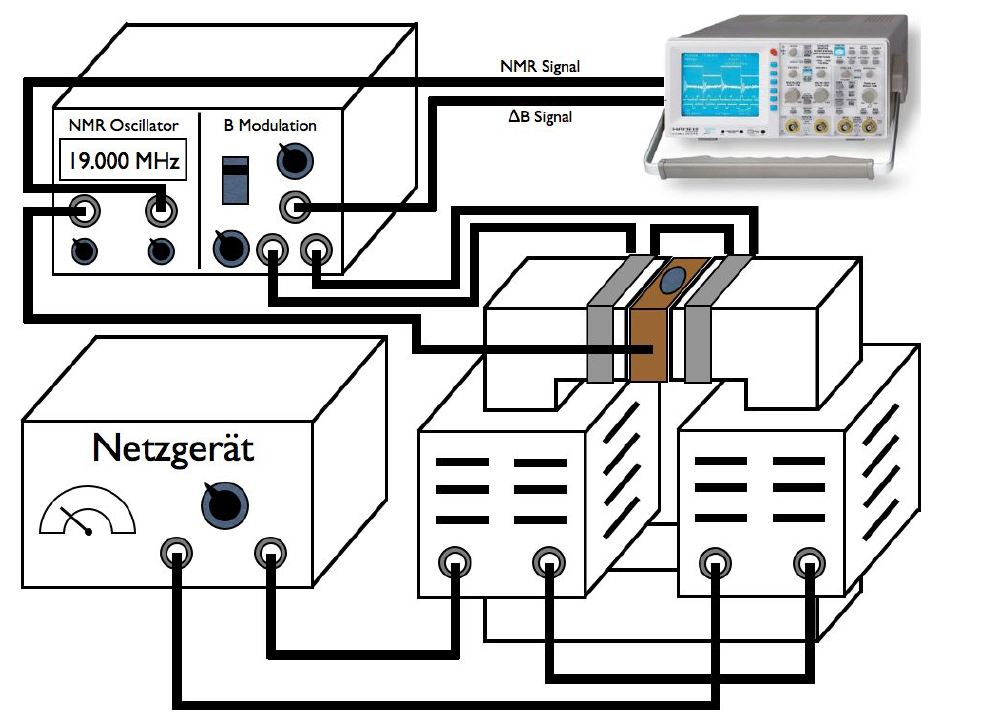
\includegraphics[scale=0.8]{Bild/Setup1}
	\centering
	\caption[Block Diagram for Setup 1]{Setup for measuring the resonance frequency with a sinus modulation.}
	\label{Exp_part1}
\end{figure}
\subsubsection{Lock-In Method}
For the second part the lock-in method is used since it is more precise duo to its lower background noise. Instead of the former absorption curve this method gives the differentiated curve. For the modulation of the magnetic field the superposition of a sinus and a sawtooth is used. Here the sawtooth is used mainly for the variance of the field while the sinus is used to create the differentiated signal since it has a similar frequency to the reference signal. The former minima of the absorption curve will now be the 'Nulldurchgang' of the signal. The moment the 'Nulldurchgang' of both measured signals overlap the correct resonance frequency is hit. Examples of both signals are shown in figure \ref{SägezahnBsp} and the setup is given in figure \ref{Exp_part2}.
\begin{figure}[ht]
	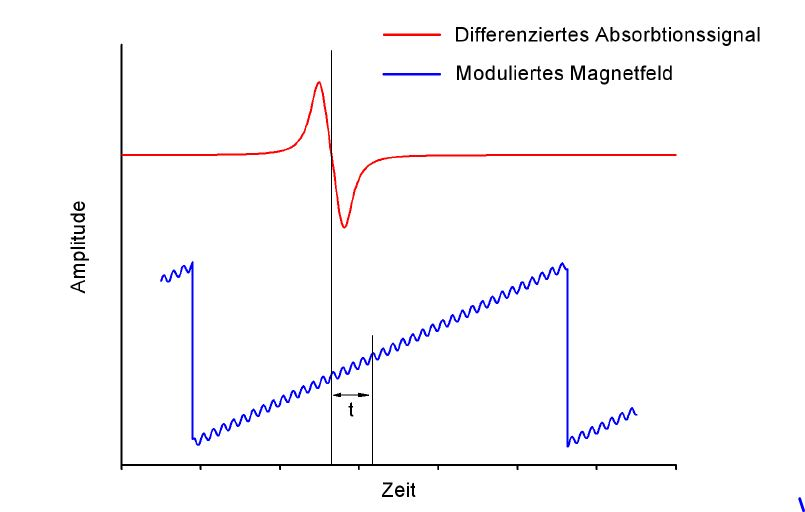
\includegraphics[scale=0.8]{Bild/BspLockIn}
	\centering
	\caption{Derived absorption signal in red. Superposition of sinus and sawtooth waves with both 'Nulldurchgängen' aligned.}
	\label{SägezahnBsp}
\end{figure}
\begin{figure}[ht]
	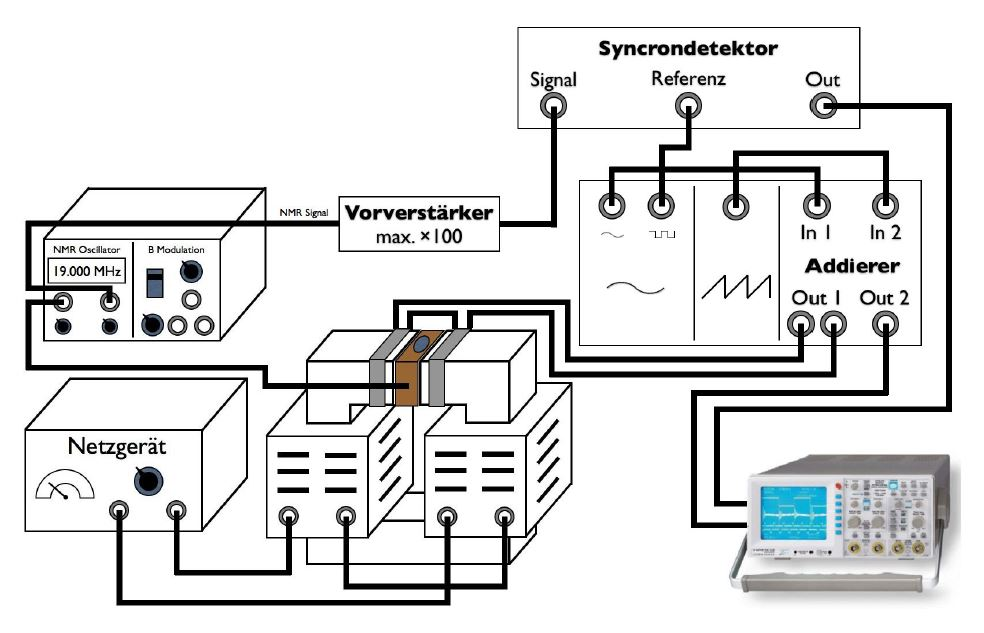
\includegraphics[scale=0.8]{Bild/Setup2}
	\centering
	\caption[Block Diagram for Setup 2]{Setup for measuring the resonance frequency with the lock-in method.}
	\label{Exp_part2}
\end{figure}


	\section{Durchführung des Versuches}
Vor der mündlichen Abfrage wurde die Messung vom Cobalt Spektrum mit dem CdTe Kristall gestartet mit einer Messzeit von einer Stunde. Nach der der mündlichen Abfrage wurde der CdTe Kristall gegen eine Silizium Diode getauscht und das zweite Cobalt Spektrum wurde mit der Messzeit von einer Stunde aufgenommen. \par
Während die obige Messung lief wurde mit den Vorbereitungen Absorptions- und Transmissionsmessungen zu Silizium gestartet. Es wurde der Strahlengang eingestellt und vorläufige Parameter des Lock-in Verstärkers gefunden.\par
Nun wurde auch das Cobalt Spektrum mittels der Silizium Diode aufgenommen, weshalb die Probe auf Americium gewechselt wurde und dessen Spektrum aufgezeichnet wurde. Die Messzeit betrug wieder eine Stunde.\par
Nach der ersten Testmessung zu Transmission und Absorption wurden die finalen Verstärkereinstellungen vorgenommen. Es wurden zwei normale Messungen und drei Untergrundmessungen aufgezeichnet: Eine ohne die Silizium Probe, eine ohne das Gitter und eine mit abgedunkeltem Spalt. Hierzu wurde das Gitter von $-90^{\circ}$ bis $+90^{\circ}$ gedreht und immer die Position des Gitters und der Widerstand der Probe sowie die Spannung des Pyrodetektors aufgezeichnet.\par
Nach Abschluss der ersten Americium Messung wurde klar, dass die Probe in der falschen Orientierung auf den Detektor platziert wurde, die Zählrate war viel niedriger als erwartet. Nachdem die Probe richtig platziert wurde, konnte die Messung mit Dauer einer Stunde erneut gestartet werden.\par
Da die Absorptions- und Transmissionsmessungen nun für Silizium abgeschlossen sind, wurde der Aufbau für die Germanium Probe vorbereitet: Das Gitter, der Filter und die Probe wurden vertauscht. Nun wurde der Verstärker für die Germanium Probe angepasst. Leider gab es zunächst Probleme, sodass man die realen Maxima erst bei maximaler Verstärkung finden konnte. Alls die Fehlersuche sich hinzog wurde beschlossen sich aufzuteilen und die Haynes und Shockley Messungen parallel durchzuführen.\par
Zunächst wurde der Offset von Glasfaser zu Elektrode bestimmt, anschließend wurde der Versuchsaufbau in Betrieb genommen. Es wurde nun die minimale Spannung  gefunden, bei welcher vermutet wurde, dass eine Auswertung der Messung in Form einer angepassten Gaußkurve möglich ist. Dann wurde in $2\,$V, später $4\,$V Schritten die Spannung erhöht bis zur maximal möglichen Spannung von $48\,$V.\par
Nun war die Messung des Americium Spektrums mit der Silizium Diode abgeschlossen und sie wurde gegen den CdTe Kristall getauscht. Anschließend wurde die letzte Messung gestartet. \par
Für das Haynes und Shockley Experiment wurden nun die Abstandsmessungen durchgeführt. Hierbei wurde zunächst die maximale Spannung an der Probe angelegt, und der Abstand so lange erhöht bis zur maximalen Distanz, bei welcher es für möglich gehalten wurde, eine Auswertung durchzuführen. Diese lag bei $9\,$mm auf der angebrachten Skala. Der Abstand wurde immer um einen mm zwischen den gespeicherten Messungen reduziert, bis zum minimalen Abstand von $2\,$mm. Es wurde nun noch einmal der Offset zwischen Glasfaser und Elektrode bestimmt, welcher jetzt $3.6\,$mm betrug. \par
Währenddessen wurde der Strahlenverlauf der Absorptions- und Transmissionsmessungen angepasst, sodass hier auch die oben erwähnten Messungen aufgenommen werden konnten.
	\include{Kapitel/AnalyseV1}
	\section{Auswertung von Haynes \& Shockley}
\subsection{Messung bei Konstanter Abstand}
	Als erstes wurden die einzelnen gemessenen Datenreihen geplottet und mit einer Gaußschen Normalverteilung gefittet. Die verwendete Form ist in Gleichung \ref{Gaus} zu finden.
	\begin{equation}
		f(x) = A \frac{1}{\sqrt{2\pi \sigma^2}} 	\exp\left(-\frac{1}{2}\frac{(x-x_c)^2}{\sigma^2}\right)+h
		\label{Gaus}
	\end{equation}
	Hierfür wurde das Python Paket \verb|scipy.optimize| mit der Funktion \verb|curve_fit| verwendet. Die Bilder der Messungen sind im Anhang.
	Die Erhaltenen Parameter wurden ohne Offset $h$ abgebildet in Abbildung \ref{SpannungGaus} dargestellt.	Wenn man die Gaußkurve mit der Differentialgleichung \ref{DifferentialGL} welche die Bewegung der Elektronenwolken in Halbleiter beschriebt, vergleicht
	\begin{equation}
		c(t,x)=C\exp\left(-\frac{t}{\tau_n}\right)\cdot\exp\left(-\frac{(x-\mu_nEt	)^2}{4D_nt}\right)
		\label{DifferentialGL}
	\end{equation}
	erhält man folgende Gleichungen für die einzelnen Parameter der Gaußkurve \ref{Gaus}:
	\begin{equation}
		x_c(t)=\mu_nEt \qquad A(t)=\exp\left(-\frac{t}{\tau_n}\right) \qquad \sigma(t)^2=2D_nt
	\end{equation}
	Hierbei sind $\mu_n$ die Beweglichkeit der Elektronenwolken, $\tau_n$ ihre Lebenszeit und $D_n$ die Diffusionskonstante.\par
	\FloatBarrier
	\begin{figure}[ht]
		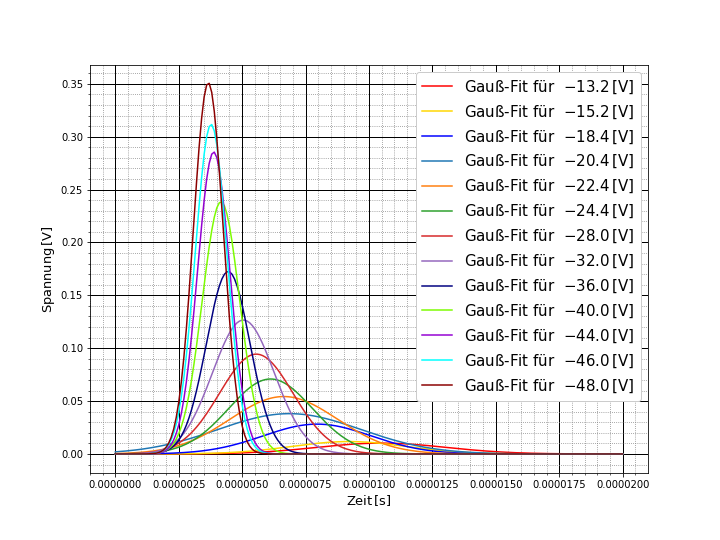
\includegraphics[scale=0.45]{Bild/V2Abstand1}
		\centering
		\caption[Darstellung der Gaußkurven bei konst. Abstand]{Gemeinsame Darstellung der Gaußkurven bei konstanten Abstand ohne Offset nebeneinander.}
		\label{SpannungGaus}
	\end{figure}
	\FloatBarrier
	Als erstes wird versucht die Beweglichkeit $\mu_n$ zu bestimmen. Hierfür wurde die Inverse Spannung $\frac{1}{U(t)}$ gegen die Zeit geplottet und mit einer gewichteten linearen Regression gefittet. Als Fehler wurden die Fehler der Zeit auf der y-Achse verwendet. Siehe Abbildung \ref{SpannungBew}. Das multiplizieren der Steigung $m$ mit der Länge des Halbleiters $l=3$\,cm so wie dem Abstand zwischen Laser und Nadel $d=3.6$\,mm ergibt nun die gesuchte Beweglichkeit.
	\begin{equation}
		\mu_1=ldm
	\end{equation}
	Der Fehler ergibt sich durch Gaußsche Fehlerfortpflanzung mit der Gleichung \ref{FFS1} wo bei die Fehler auf die Abstände beide auf $0.1$\,mm geschätzt wurden.
	\begin{equation}
		\sigma_{\mu_1}=\sqrt{\left(dm\sigma_l\right)^2+\left(lm\sigma_d\right)^2+\left(dl\sigma_m\right)^2}
		\label{FFS1}
	\end{equation}
	Dies ergab einen Wert von $\mu_1=\left(3.90 \pm 0.07\right) \times 10^{3}\,\frac{\text{cm}^2}{\text{Vs}}$
	Nun wurde die Lebenszeit über die Amplitude der Gaußfits bestimmt. Hierfür wurde als Amplitude $A \frac{1}{\sqrt{2\pi \sigma^2}}$ verwendet und dies gegen die Zeit geplottet. Die Datenpunkte wurden dann wie in Abbildung \ref{SpannungTau} zu sehen exponentiell gefittet mit der Form \ref{Expotentialform}.
	\begin{equation}
		f(x)=C\exp\left(-\frac{t}{\tau}\right)+h
		\label{Expotentialform}
	\end{equation}
	Für den Parameter und damit die Lebenszeit ergab sich ein Wert von $\tau_1=\left(1.28 \pm 0.08\right) \times 10^{-6}\,s$
	Nun wird die Diffusionskonstante $D_1$ bestimmt, indem $\sigma^2$ gegen die Zeit dargestellt wird und eine linearer Fit an diese Werte angepasst wird (siehe Abbildung \ref{SpannungD}). Da die Fehler auf das Sigma durch das Quadrieren relativ groß wurden wurde ein gewichteter fit mit Fehlern auf $\sigma^2$ durchgeführt. Das halbieren der Steigung des Fits ergibt für die Diffusionskonstante  $D_1=\left(3.4 \pm 0.5\right) \times 10^{-5}
	\,\frac{\text{cm}^2}{\text{s}}$.
	Die Werte sind noch einmal gemeinsam in Tabelle \ref{MesswerteV2} dargestellt, zusammen mit dem erwarteten Literaturwert.
	\FloatBarrier
	\begin{figure}[ht]
		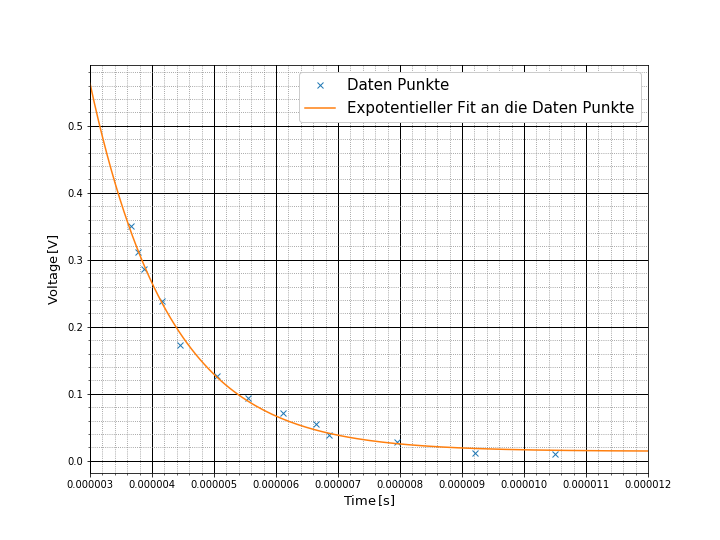
\includegraphics[scale=0.43]{Bild/V2Abstand3}
		\centering
		\caption[Exponentieller Fit der Amplituden bei konstantem Abstand]{\small Exponentieller Fit der Amplituden bei Konstantem Abstand. Fehler wurden nicht eingezeichnet, da sie nicht sinnvoll zu erkennen waren.}
		\label{SpannungTau}
	\end{figure}
	\begin{figure}[ht]
		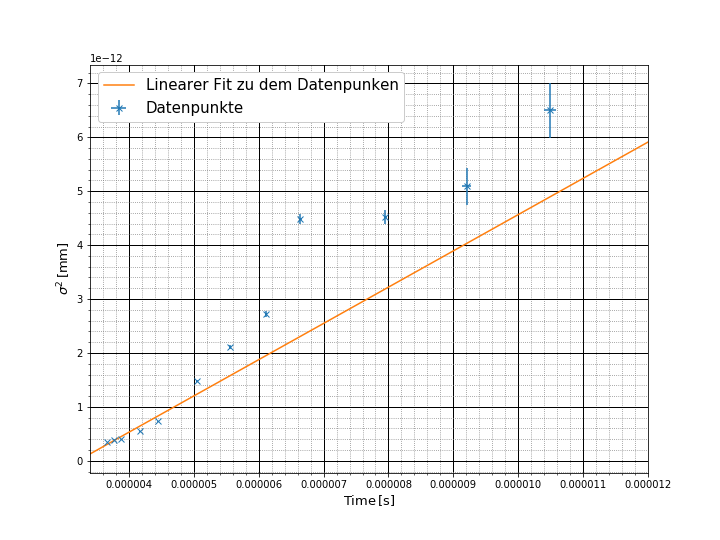
\includegraphics[scale=0.43]{Bild/V2Abstand4}
		\centering
		\caption[Fit zur Bestimmung der Diffusion bei konst. Abstand.]{\small Datenpunkte von $\sigma^2$ gegen die Zeit mit Fehlern. In orange der gerade Fit zur Bestimmung der Diffusionskonstante.}
		\label{SpannungD}
	\end{figure}
	\begin{figure}[ht]
		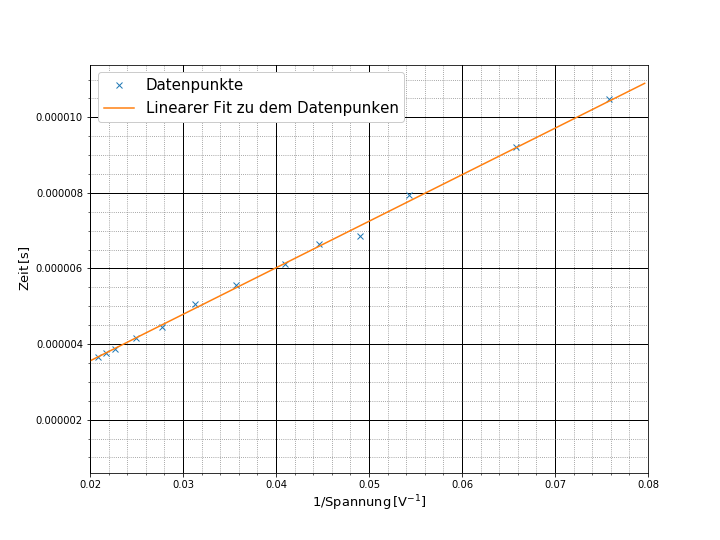
\includegraphics[scale=0.5]{Bild/V2Abstand2}
		\centering
		\caption[Linearer Fit zur Bestimmung der Beweglichkeit bei konst. Abstand]{Linearer Fit zur Bestimmung der Beweglichkeit bei konst. Abstand. Fehler wurden nicht beigefügt, da diese sich nicht sinnvoll darstellen ließen.}
		\label{SpannungBew}
	\end{figure}
	\FloatBarrier
	\newpage
	\subsection{Messung bei Konstante Spannung}
	Für die Messung mit Konstanter Spannung werden wie zuvor die Daten mit der Gleichung \ref{Gaus} gefittet und sind in Abbildung \ref{Abstand1} ohne Offset dargestellt.\par
	\FloatBarrier
	\begin{figure}[ht]
		\includegraphics[scale=0.5]{Bild/V2Spannung1}
		\centering
		\caption[Darstellung der Gaußkurven bei konst. Spannung]{\small Gemeinsame Darstellung der Gaußkurven bei konstanter Spannung ohne Offset nebeneinander.}
		\label{Abstand1}
	\end{figure}
	\FloatBarrier
	Als nächstes wurde die Beweglichkeit $\mu_2$ bestimmt indem der gemessene Abstand zwischen Nadel und Laser gegen die Zeit gefittet, welche die Elektronenwolke benötigte. Hierbei wurden die Fehler auf die Zeit mitberücksichtigt. Die Steigung $m$ erhält man mit Gleichung \ref{AbstandBesch}.
	\begin{equation}
		\mu_2=\frac{1}{mE} \qquad \qquad \sigma_{mu_2}=\sqrt{\left(\frac{\sigma_{m}}{m^2E}\right)^2+\left(\frac{\sigma_{E}}{mE^2}\right)}
		\label{AbstandBesch}
	\end{equation}
	$E$ kann hier über die angelegte Spannung $U=(48\pm0.5)\,$V und die Länge $l=3\pm0.1\,$cm mit Gleichung \ref{E} bestimmt werden.
	\begin{equation}
		E=\frac{U}{l} \qquad \qquad \sigma_E=\sqrt{\left(\frac{\sigma_U}{l}\right)^2+\left(\frac{U\sigma_l}{l^2}\right)^2}
		\label{E}
	\end{equation}
	Damit ergibt sich für $\mu_2=(3136 \pm 32)\,\frac{\text{cm}^2}{Vs}$.\par
	\begin{figure}[ht]
		\includegraphics[scale=0.5]{Bild/V2Spannung2}
		\centering
		\caption[Linearer Fit zur Bestimmung der Beweglichkeit bei konst. Spannung]{\small Linearer Fit zur Bestimmung der Beweglichkeit bei konst. Spannung. Fehler wurden nicht beigefügt, da diese sich nicht sinnvoll darstellen ließen.}
		\label{Abstand}
	\end{figure}
	Danach wird wie bei dem Konstanter Spannung die Lebenszeit wie zuvor über die Amplitude bestimmt. Hierzu wird Gleichung \ref{Expotentialform} benutzt wie in Abbildung \ref{AbstandTau} dargestellt. Für die Lebenszeit ergibt sich dadurch ein Wert von $\tau_2= \left(5.9 \pm 1.0\right) \times 10^{-6}\,s$.\par
	\begin{figure}[ht]
		\includegraphics[scale=0.5]{Bild/V2Spannung3}
		\centering
		\caption[Exponentieller Fit der Amplituden bei konstanter Spannung]{\small Exponentieller Fit der Amplituden bei Konstanter Spannung. Fehler wurden nicht eingezeichnet, da sie nicht sinnvoll zu erkennen waren.}
		\label{AbstandTau}
	\end{figure} 
	Für die Diffusionskonstante wird wieder der Parameter $\sigma^2$ mit Fehlern gegen die Zeit aufgetragen und mit einem gewichteten Fit angepasst. Beide sind in Abbildung \ref{AbstandD}. Es ergibt sich durch halbieren der Steigung ein Wert von $D_2=\left(2.8 \pm 0.7\right) \times 10^{-6}$. Die Werte sind noch einmal gemeinsam in Tabelle \ref{MesswerteV2} dargestellt zusammen mit dem erwarteten Literaturwert.
	\begin{figure}[ht]
		\includegraphics[scale=0.5]{Bild/V2Spannung4}
		\centering
		\caption[Fit zur Bestimmung der Diffusion bei konst. Spannung.]{\small Datenpunkte von $\sigma^2$ gegen die Zeit mit Fehlern. In orange der gerade Fit zur Bestimmung der Diffusionskonstante.}
		\label{AbstandD}
	\end{figure}
	\begin{table}[ht]
		\begin{Dtabular}[1.1]{|c|c|c|c|}
			\hline
			&Beweglichkeit $\mu$ [$\frac{\text{cm}^2}{\text{Vs}}$]&Lebenszeit $\tau$ [$\mu$s]& Diffusion $D$ [$\frac{\text{cm}^2}{\text{s}}$]\\
			\hline
			Messung bei konst. Abstand&$\left(3900 \pm 70\right)$&$\left(1.28 \pm 0.08\right)$&$\left(3.4 \pm 0.5\right) \times 10^{-5}$\\
			\hline
			Messung bei konst. Spannung&$(3136 \pm 32)$&$\left(5.9 \pm 1.0\right)$&$\left(2.8 \pm 0.7\right) \times 10^{-6}$\\
			\hline
			Literaturwert&$3900$&$(45\pm2)$&$101$\\
			\hline
		\end{Dtabular}
		\centering
		\caption{Messwerte von Versuchsteil 2 mit Literaturwerten\cite{anleitung}}
		\label{MesswerteV2}
	\end{table}
	\section{Auswertung von Halbleiter Experiment}
Im Versuchsteil 3 wurden die Energiespektren von $^{241}$Am und $^{57}$Co mit zwei unterschiedlichen Detektoren aufgenommen. Für die Auswertung wurden hier der $122.06\,$keV so wie der $136.47\,$keV Photopeak von Cobalt so wie der $59.5\,$keV Peak von Americium mit einer Gaußkurve wie in Gleichung \ref{Gaus} gefittet. Die Peaks so wie die dazugehörigen Anpassungen für $^{57}$Co sind in Abbildung \ref{CoS} und \ref{CoC} zu sehen. Die für Americium sind in Abbildung \ref{AmS} und \ref{AmC} zu finden. Die gesamten Spektren sind im Anhang.\par
\begin{figure}[ht]
	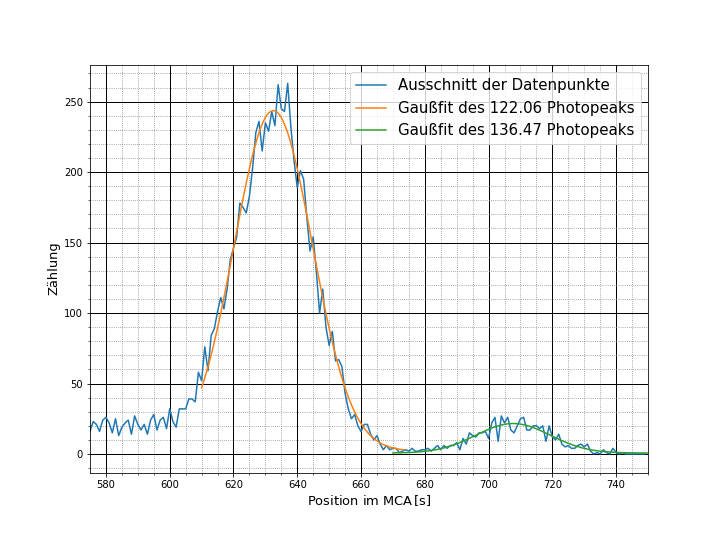
\includegraphics[scale=0.5]{Bild/CS.png}
	\centering
	\caption[V3 $122.06\,$keV und $136.47\,$keV Peaks mit Silizium Detektor]{Gaußfit für einen denn Datenbereich der $122.06\,$keV und $136.47\,$keV Photopeaks mit dem Silizium Detektor.}
	\label{CoS}
\end{figure}
\begin{figure}[ht]
	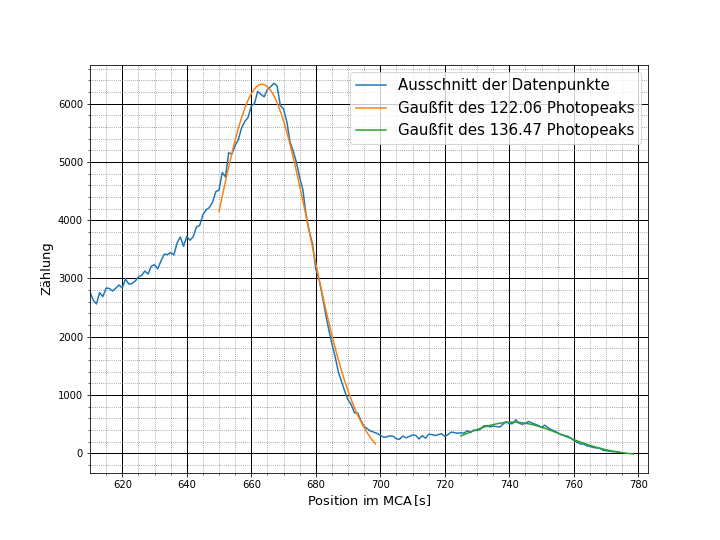
\includegraphics[scale=0.5]{Bild/CC.png}
	\centering
	\caption[V3 $122.06\,$keV und $136.47\,$keV Peaks mit CdTe Detektor]{Gaußfit für einen denn Datenbereich der $122.06\,$keV und $136.47\,$keV Photopeaks mit dem CdTe Detektor.}
	\label{CoC}
\end{figure}
\begin{figure}[ht]
	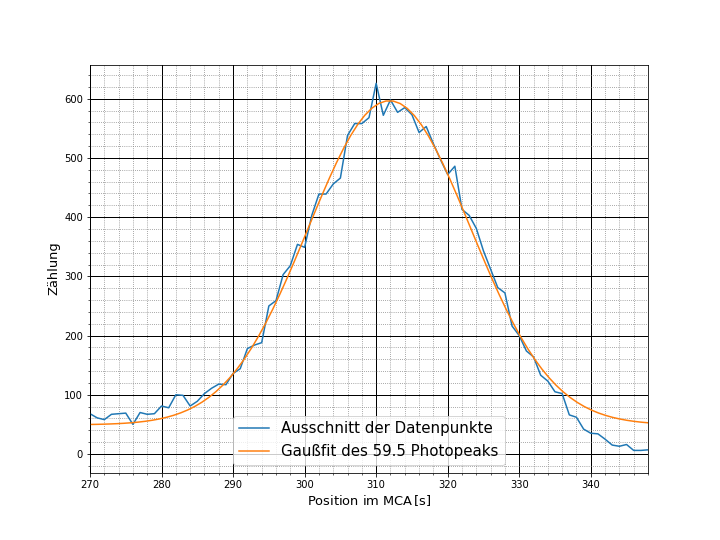
\includegraphics[scale=0.5]{Bild/AS.png}
	\centering
	\caption[V3 $59.5$\,keV Peaks mit Silizium Detektor]{Gaußfit für einen denn Datenbereich der $59.5$\,keV Photopeaks mit dem Silizium Detektor.}
	\label{AmS}
\end{figure}
\begin{figure}[ht]
	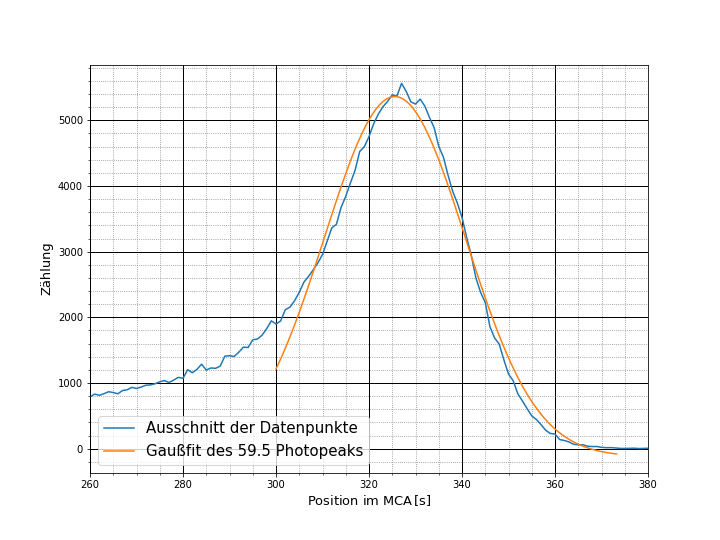
\includegraphics[scale=0.5]{Bild/AC.png}
	\centering
	\caption[V3 $59.5$\,keV Peaks mit CdTe Detektor]{Gaußfit für einen denn Datenbereich der $59.5$\,keV Photopeaks mit dem CdTe Detektor.}
	\label{AmC}
\end{figure}
\FloatBarrier
Die Position der Peaks welche die Kanalnummer des MCA's ist kann nun mit Hilfe der bekannten Energien geeicht werden, indem man separat für beide Detektoren Energie gegen Position aufträgt und die Werte dann linear anpasst. Hierbei wurde ein gewichteter Fit verwendet welche die Fehler auf die Position der Peaks berücksichtigte. Die Werte so wie die angepasste Kurve sind in Abbildung \ref{Eichung} zu sehen. Die erhaltenen Gleichungen für denn Zusammenhang zwischen Kanal und Energie sind:\par
\begin{equation*}
	f(E)_{Kanal} = (5.3988\pm 0.0010)\,\frac{1}{\text{keV}}E+(4.33\pm 0.10)
\end{equation*}
\begin{equation*}
f(E)_{Kanal} = (5.128\pm 0.008)\,\frac{1}{\text{keV}}E+(6.7\pm 0.8)
\end{equation*}
\begin{figure}[ht]
	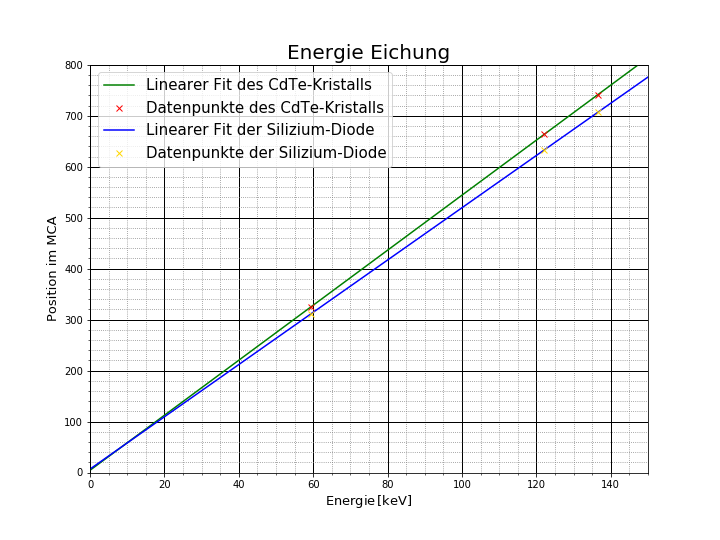
\includegraphics[scale=0.5]{Bild/Eichung.png}
	\centering
	\caption[Eichung für beide Detektoren]{Geraden zur Eichung der beiden Detektoren. In blau die Eichung für den Silizium Detektor und in grün für den CdTe Detektor. Fehler sind nicht mit eingezeichnet da sie zu klein waren um sie sinnvoll darzustellen.}
	\label{Eichung}
\end{figure}
Nun wird mit das Absorptionsverhältnis der beiden Detektoren bei unterschiedlichen Energien bestimmt. Dafür müssen die aus den Fit bestimmten Amplituden erst einmal aktive Fläche normiert werden und dann durcheinander geteilt wie in Gleichung \ref{Abs} dargestellt:
\begin{eqnarray}
\frac{Abs_{\text{Si}}}{Abs_{\text{CdTe}}}=\frac{\nicefrac{A_{\text{Si}}}{a_{\text{Si}}}}{\nicefrac{A_{\text{CdTe}}}{a_{\text{CdTe}}}}
\label{Abs}
\end{eqnarray}
Die Fläche des CdTe Detektors beträgt $a_\text{CdTe}=23\,\text{mm}^2$ und die des Si Detektors $a_{\text{Si}}=100\,\text{mm}^2$. Die erhaltenen Werte sind zusammen mit den Literaturwerten aus der Anleitung\cite{anleitung} in Tabelle \ref{MesswerteV3_1} zu finden.
Als letztes wird die Relative Energieauflösung der einzelnen Peaks bestimmt. Zur Berechnung wird die Halbwertsbreite verwendet wodurch sich folgende Gleichung ergibt:
\begin{equation}
	RER(E)=\frac{FWHM}{E}\approx\frac{2.35\sigma(E)}{E}
\end{equation}
Die erhaltenen Werte sind in Tabelle \ref{MesswerteV3_2} zu finden.
\begin{table}[ht]
	\begin{Dtabular}[1.1]{|c|c|c|}
		\hline
		Photopeak Energie [keV]&Berechnete Werte [\%] &Literaturwerte [\%]\\
		\hline
		$59.5$&$1.28 \pm 0.07$&$1,40$\\
		\hline
		$122.06$&$0.58 \pm 0.05$&$1,83$\\
		\hline
		$136.47$&$0.45 \pm 0.06$&$2,00$\\
		\hline
	\end{Dtabular}
	\centering
	\caption{Absorptionsverhältnis von Versuchsteil 3 mit Literaturwerten\cite{anleitung}}
	\label{MesswerteV3_1}
\end{table}
\begin{table}[ht]
	\begin{Dtabular}[1.1]{|c|c|c|c|}
		\hline
		Detektor und Energie&Energieauflösung\\
		\hline
		Silizium $59.5$&$0.449 \pm 0.007$\\
		\hline
		Silizium $122.06$&$0.236 \pm 0.005$\\
		\hline
		Silizium $136.47$&$0.200 \pm 0.010$\\
		\hline
		CdTe $59.5$&$0.600 \pm 0.012$\\
		\hline
		CdTe $122.06$&$0.285 \pm 0.007$\\
		\hline
		CdTe $136.47$&$0.272 \pm 0.010$\\
		\hline
	\end{Dtabular}
	\centering
	\caption{Energieauflösung von Versuchsteil 2 mit Literaturwerten\cite{anleitung}}
	\label{MesswerteV3_2}
\end{table}	
	\section{Zusammenfassung und Diskussion zum Versuchsteil 2}
Im Versuchsteil 2 ging es darum die Elektronenwolken innerhalb eines Halbleiters zu untersuchen. Hierfür wurden ein $3$cm langer Germanium Block genutzt. Zur Messung wurde einmal der Abstand zwischen Laser und Nadel verändert und einmal die am Germanium angelegte Spannung.
Die berechneten Werte sind die Lebensdauer, Beweglichkeit so die Diffusion der Wolken und sind in Tabelle \ref{MesswerteV2} zu finden. Zum Vergleich der Werte mit dem Literaturwert wurde die Gleichung \ref{vgl} verwendet. Die Werte sind in Tabelle \ref{VGLV2} notiert.
\begin{equation}
	t=\frac{x_{Mess}-x_{Literatur}}{\sigma_{x_{Messung}}}
	\label{vgl}
\end{equation}
\FloatBarrier
\begin{table}[ht]
	\begin{Dtabular}[1.1]{|c|c|c|}
		\hline
		&t bei konst. Abstand $[\sigma]$&t bei konst. Spannung $[\sigma]$\\
		\hline
		$\mu$ &$0.0$&$23.875$\\
		\hline
		$\tau$ &$546.5$&$39.1$\\
		\hline
		$D$ &$202.0$&$144.3$\\
		\hline
	\end{Dtabular}
	\centering
	\caption[Vergleichswerte V2]{Vergleichswerte der Berechneten Werte mit dem Literaturwerten über Gleichung \ref{vgl}}
	\label{VGLV2}
\end{table}
Wenn man sich diese Werte anschaut passen bis auf den Wert bei $\mu$ mit konstantem Abstand keine der Werte überein. Die große Abweichung bei der Lebenszeit kann man damit erklären, dass die freien Elektronen tiefer in der Germanium Probe erzeugt werden. Gittereffekte naher der Oberfläche können daher zu ein Grund für die starke Verkürzung der Lebenszeit sein.
	\section{Zusammenfassung und Diskussion zum Versuchsteil 3}
Im Versuchsteil 3 ging es um Halbleiterdetektoren. Hierbei wurde eine Silizium Diode und ein CdTe Kristall verwendet. Mit ihnen wurden die Energiespektren von $^57$Co und $^241$Am aufgezeichnet. Mit diesen Spektren wurde eine Energieeichung durchgeführt und dann die Energieauflösung der einzelnen Peaks so, wie das Absorptionsverhältnis der beiden Detektoren bei den Unterschiedlichen Peaks bestimmt.\par
Wenn man sich die Eichungen anschaut scheinen die Messwerte sehr gut zueinander zu passen, es fällt jedoch auf, dass die geraden eine Abweichung der Steigung voneinander haben, was zeigt, dass eine individuelle Kalibrierung sinnvoll ist.\par

Wenn man sich die Werte für die Absorptionsverhältnisse anschaut (siehe Tabelle \ref{MesswerteV3_1}) fällt auf das es einen großen unterschied zwischen denen bei höheren Energien also den beiden $^57$Co Photopeaks der Wert geringer ist als bei der niedrigeren vom $59.5\,$keV Peak von Americium. Dies steht etwas im Widerspruch zu den Literaturwerten bei denen das Absorptionsverhältnis für höhere Energien größer ist. Gründe dafür können Abweichungen der Herstellerangaben sein oder ein großer Verlust an Signalstärke durch Ladungsrekombination verloren haben, dass sie dem ursprünglichen Peak nicht mehr zugeschrieben werden können. Auch wurde die Absorption in der Epoxid-Schicht so wie der Si02-Schicht der Silizium-Diode nicht mitberücksichtigt.\par
Bei Betrachtung der Energieauflösung in Tabelle \ref{MesswerteV3_2} fällt auf, dass die Auflösung des Silizium Detektors besser ist als die des CdTe Detektors. Auch scheint sich die Auflösung bei höheren Energien merklich zu verbessern. So scheinen sich die Photopeaks von Cobalt fast doppelt so gut auflösen wie beim $59.5$\,keV Peak von Americium.

	
	
	
	
	\section{Tabellen}
	\listoftables
	\section{Bilder}
	\listoffigures
	\section{Bibliograpy}
	\bibliographystyle{plain}
	\bibliography{Quellen}
	\addcontentsline{toc}{section}{Literatur}
	\section{Anhang}
	\begin{figure}
	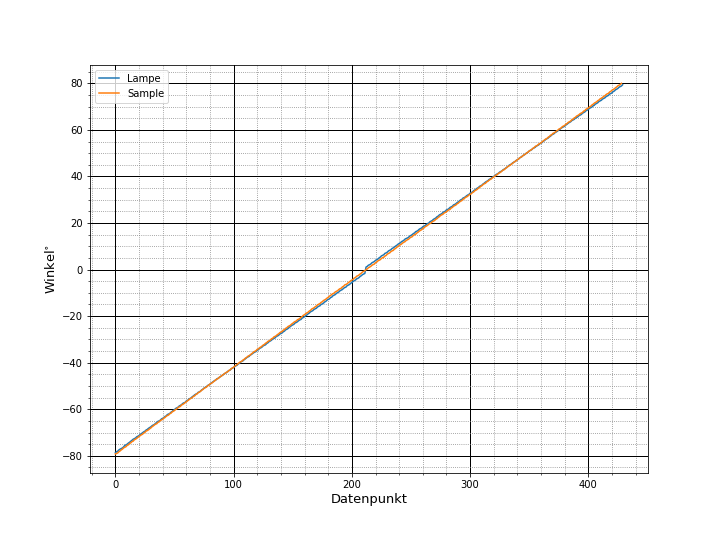
\includegraphics[scale=0.5]{Bilder/anhang/korrektur_channels_2}
	\centering
	\caption[Korrigierter Lampendatensatz 2. Silizium messung]{\small Auftragung der gemessenen Winkel für die Lampenmessung und erste Silizium Messung nach der Korrektur. Beide stimmen in den relevanten Bereichen bei ca. $30^{\circ}-40^{\circ}$ weitgehend überein.}
\end{figure}
\begin{figure}
	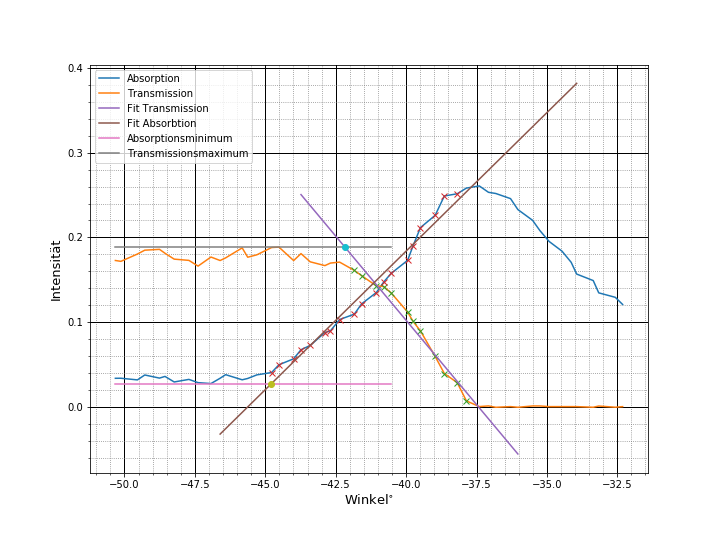
\includegraphics[scale=0.5]{Bilder/anhang/si_2_l}
	\centering
	\caption[Geraden Anpassungen 2. Silizium Messung links]{\small Auftragung von Intensität der normalisierten Datenreihen gegen die  Winkel in der Nähe der Stelle Gleichwahrscheinlicher Absorption und Transmission bei Winkeln kleiner als $0^\circ$. Es sind zusätzlich die angepassten Geraden zur Absorption und Transmission eingezeichnet. Die Horizontalen wurden durch die Maxima der dahinterliegenden Datenpunkte bestimmt. Die Schnittpunkte der Geraden mit ihren jeweiligen Horizontalen sind auch eingezeichnet.}
\end{figure}
\begin{figure}
	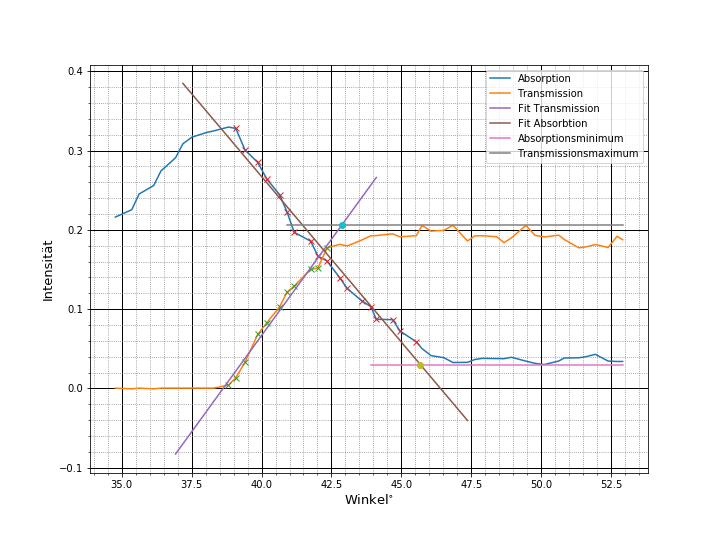
\includegraphics[scale=0.5]{Bilder/anhang/si_2_r}
	\centering
	\caption[Geraden Anpassungen 2. Silizium Messung rechts]{\small Auftragung von Intensität der normalisierten Datenreihen gegen die  Winkel der zweiten Silizium Messung in der Nähe der Stelle Gleichwahrscheinlicher Absorption und Transmission bei Winkeln größer als $0^\circ$. Es sind zusätzlich die angepassten Geraden zur Absorption und Transmission eingezeichnet. Die Horizontalen wurden durch die Maxima der dahinterliegenden Datenpunkte bestimmt. Die Schnittpunkte der Geraden mit ihren jeweiligen Horizontalen sind auch eingezeichnet.}
	\label{si_2_r}
\end{figure}
\begin{figure}
	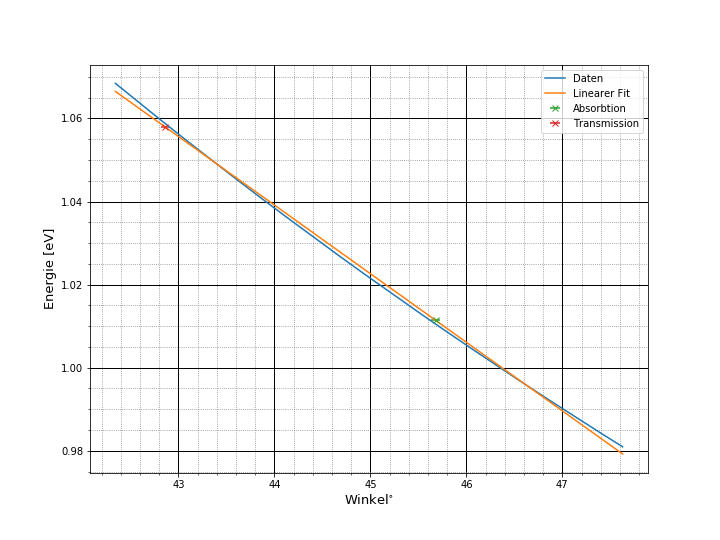
\includegraphics[scale=0.5]{Bilder/anhang/si_2_l_energie}
	\centering
	\caption[Energiebestimmung 2. Si Messung links]{\small Auftragung der Energie gegen den Winkel der zweiten Silizium Messung. Die angepasste Gerade und die beiden Schnittpunkte sind auch eingetragen.}
\end{figure}
\begin{figure}
	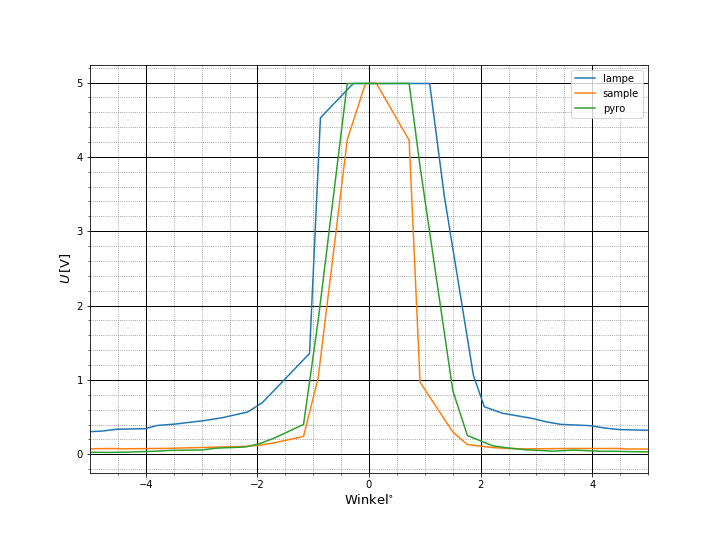
\includegraphics[scale=0.5]{Bilder/anhang/winkelkorrektur_vorher}
	\centering
	\caption[Mittelpunkt der 2. Si Messung vor Winkelkorrektur]{\small Auftragung der Intensität gegen den Winkel der zweiten Silizium Messung in der Nähe von $0^\circ$ vor der Korrektur.}
\end{figure}
\begin{figure}
	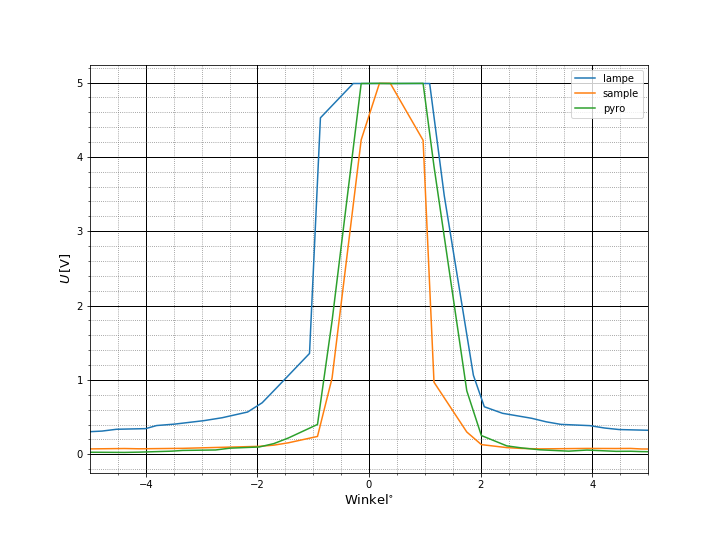
\includegraphics[scale=0.5]{Bilder/anhang/winkelkorrektur_nachher}
	\centering
	\caption[Mittelpunkt der 2. Si Messung vor Winkelkorrektur]{\small Auftragung der Intensität gegen den Winkel der zweiten Silizium Messung in der Nähe von $0^\circ$ nach der Korrektur.}
\end{figure}
\begin{figure}
	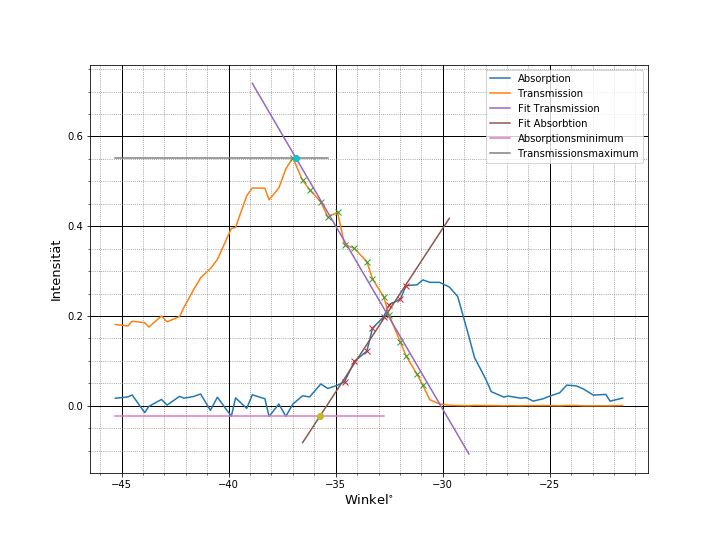
\includegraphics[scale=0.5]{Bilder/anhang/ge_r}
	\caption[Geraden Anpassungen Germanium Messung links]{\small Auftragung von Intensität der normalisierten Datenreihen von Germanium gegen die  Winkel in der Nähe der Stelle Gleichwahrscheinlicher Absorption und Transmission bei Winkeln größer als $0^\circ$. Es sind zusätzlich die angepassten Geraden zur Absorption und Transmission eingezeichnet. Die Horizontalen wurden durch die Maxima der dahinterliegenden Datenpunkte bestimmt. Die Schnittpunkte der Geraden mit ihren jeweiligen Horizontalen sind auch eingezeichnet.}
\end{figure}
\begin{figure}
	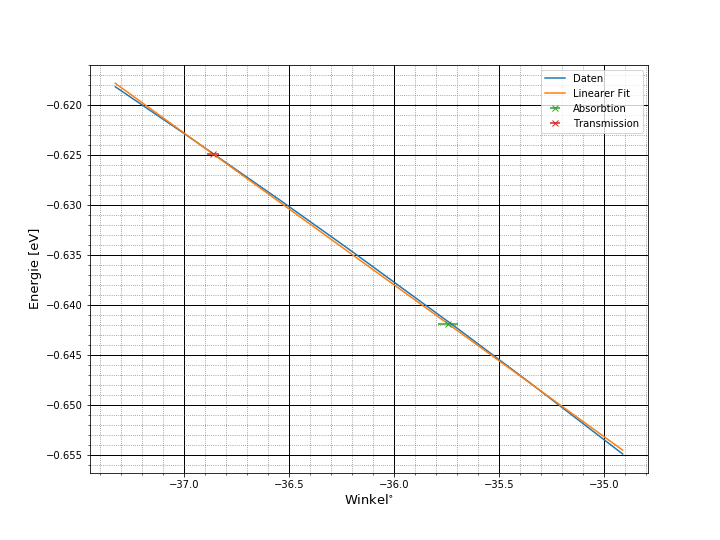
\includegraphics[scale=0.5]{Bilder/anhang/ge_l_energie}
	\centering
	\caption[Energiebestimmung Ge Messung links]{\small Auftragung der Energie gegen den Winkel der Germanium Messung. Die angepasste Gerade und die beiden Schnittpunkte sind auch eingetragen.}
\end{figure}


\begin{figure}
	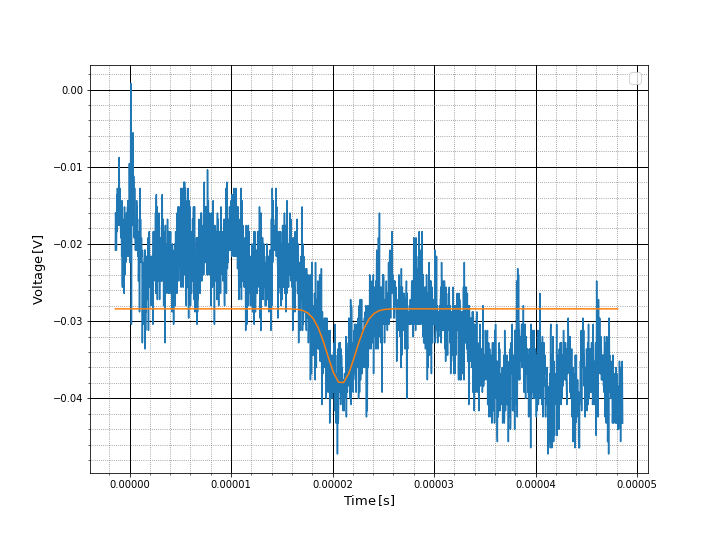
\includegraphics[scale=0.5]{Bild/S1}
	\centering
	\caption[Gaußfit an Messung bei Konst. Spannung 1]{Gaußfit an die Messungen der Elektronenwolken bei einer Spannung von $48\,$V und einem Abstand zwischen Nadel und Lase von $10.6$\,mm.}
\end{figure}
\begin{figure}
	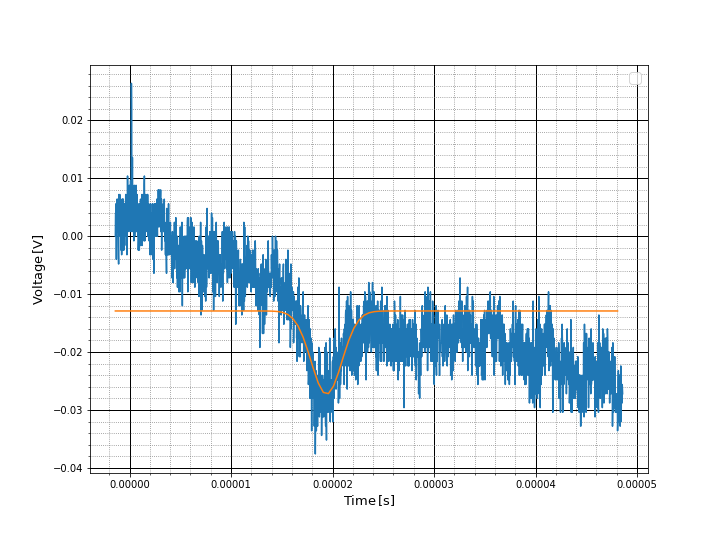
\includegraphics[scale=0.5]{Bild/S2}
	\centering
	\caption[Gaußfit an Messung bei Konst. Spannung 2]{Gaußfit an die Messungen der Elektronenwolken bei einer Spannung von $48\,$V und einem Abstand zwischen Nadel und Lase von $9.6$\,mm.}
\end{figure}
\begin{figure}
	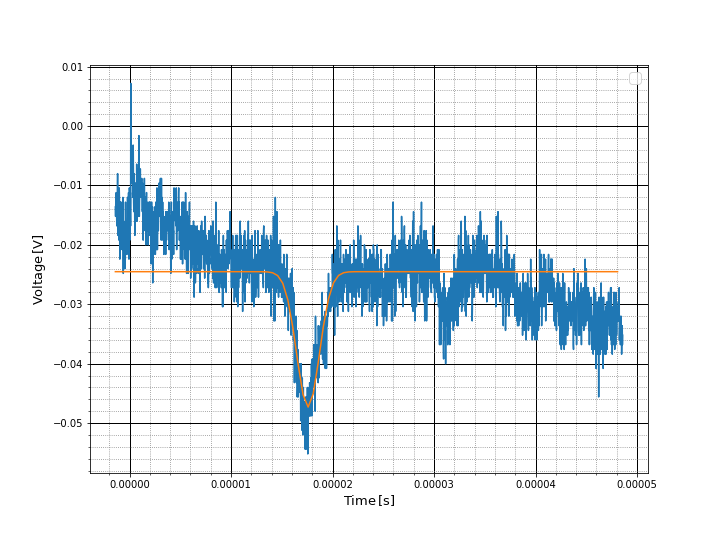
\includegraphics[scale=0.5]{Bild/S3}
	\centering
	\caption[Gaußfit an Messung bei Konst. Spannung 3]{Gaußfit an die Messungen der Elektronenwolken bei  einer Spannung von $48\,$V und einem Abstand zwischen Nadel und Lase von $8.6$\,mm.}
\end{figure}
\begin{figure}
	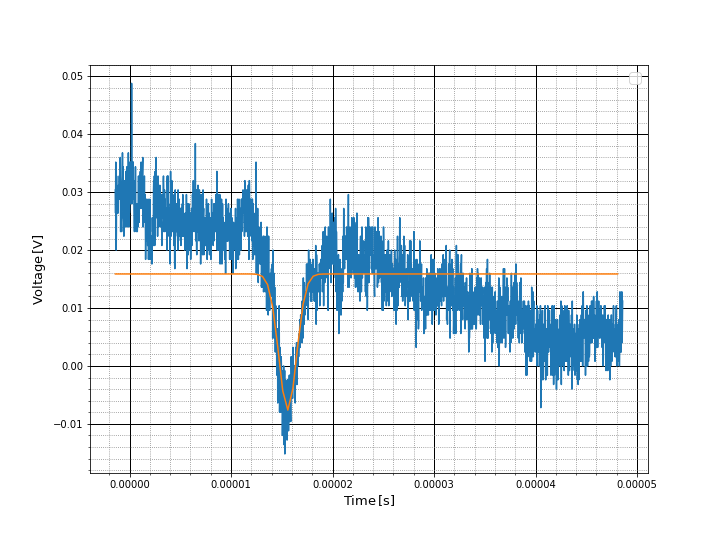
\includegraphics[scale=0.5]{Bild/S4}
	\centering
	\caption[Gaußfit an Messung bei Konst. Spannung 4]{Gaußfit an die Messungen der Elektronenwolken bei  einer Spannung von $48\,$V und einem Abstand zwischen Nadel und Lase von $7.6$\,mm.}
\end{figure}
\begin{figure}
	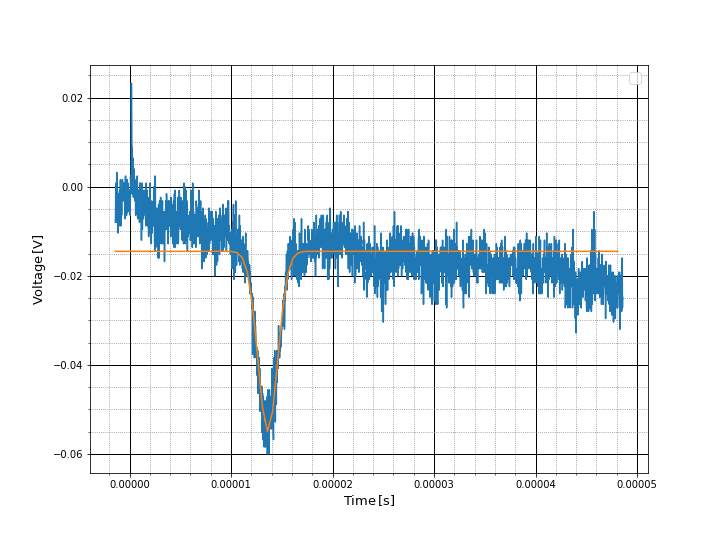
\includegraphics[scale=0.5]{Bild/S5}
	\centering
	\caption[Gaußfit an Messung bei Konst. Spannung 5]{Gaußfit an die Messungen der Elektronenwolken bei einer Spannung von $48\,$V und einem Abstand zwischen Nadel und Lase von $6.6$\,mm.}
\end{figure}
\begin{figure}
	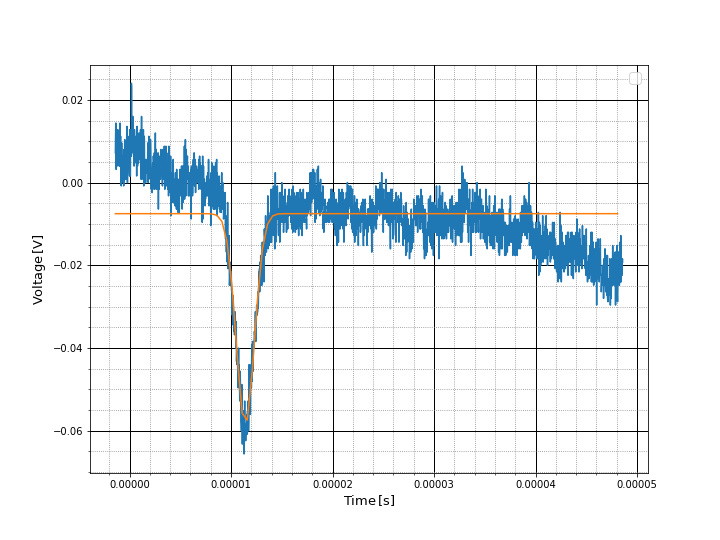
\includegraphics[scale=0.5]{Bild/S6}
	\centering
	\caption[Gaußfit an Messung bei Konst. Spannung 6]{Gaußfit an die Messungen der Elektronenwolken bei einer Spannung von $48\,$V und einem Abstand zwischen Nadel und Lase von $5.6$\,mm.}
\end{figure}
\begin{figure}
	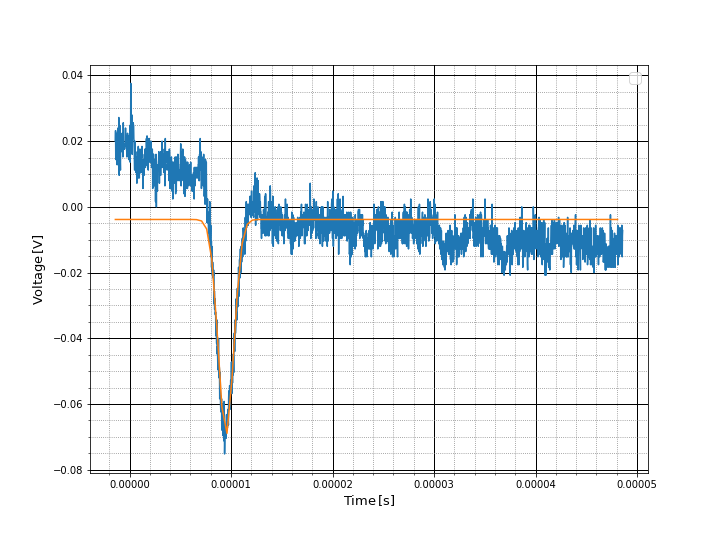
\includegraphics[scale=0.5]{Bild/S7}
	\centering
	\caption[Gaußfit an Messung bei Konst. Spannung 7]{Gaußfit an die Messungen der Elektronenwolken bei einer Spannung von $48\,$V und einem Abstand zwischen Nadel und Lase von $4.6$\,mm.}
\end{figure}
\begin{figure}
	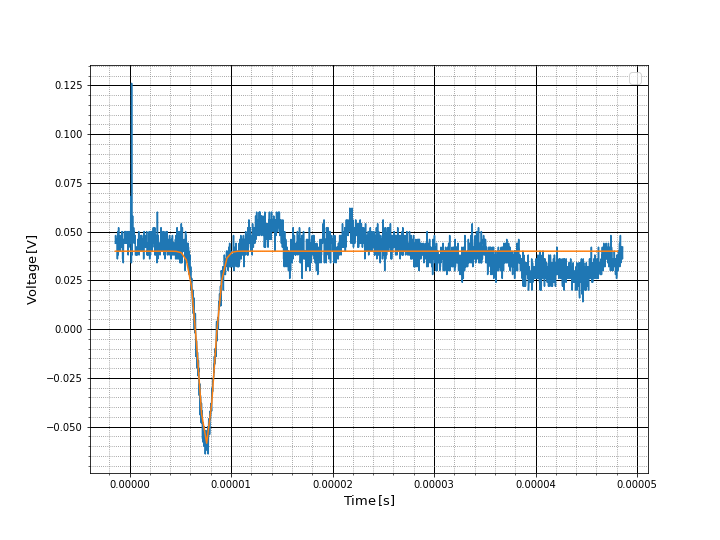
\includegraphics[scale=0.5]{Bild/S8}
	\centering
	\caption[Gaußfit an Messung bei Konst. Spannung 8]{Gaußfit an die Messungen der Elektronenwolken bei einer Spannung von $48\,$V und einem Abstand zwischen Nadel und Lase von $3.6$\,mm.}
\end{figure}

%Andere Messreihe

\begin{figure}
	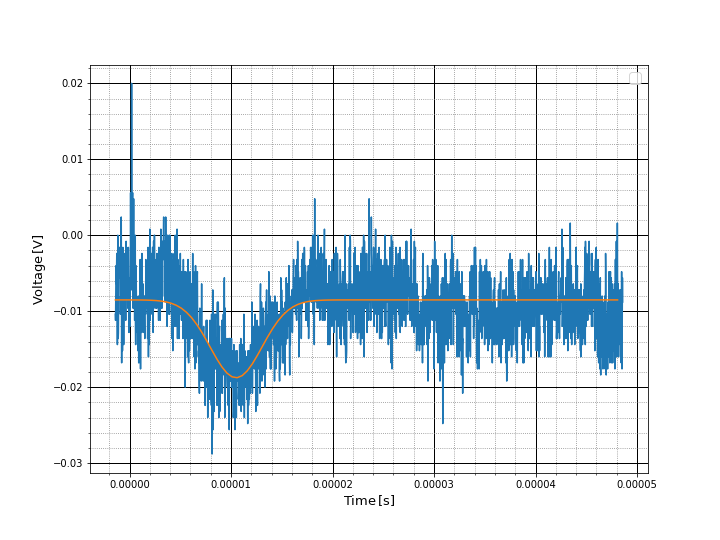
\includegraphics[scale=0.5]{Bild/A1}
	\centering
	\caption[Gaußfit an Messung bei Konst. Abstand]{Gaußfit an die Messungen der Elektronenwolken bei Konstantem Abstand von $3.6$\,mm und einer Spannung von $-13.2$\,V}
\end{figure}
\begin{figure}
	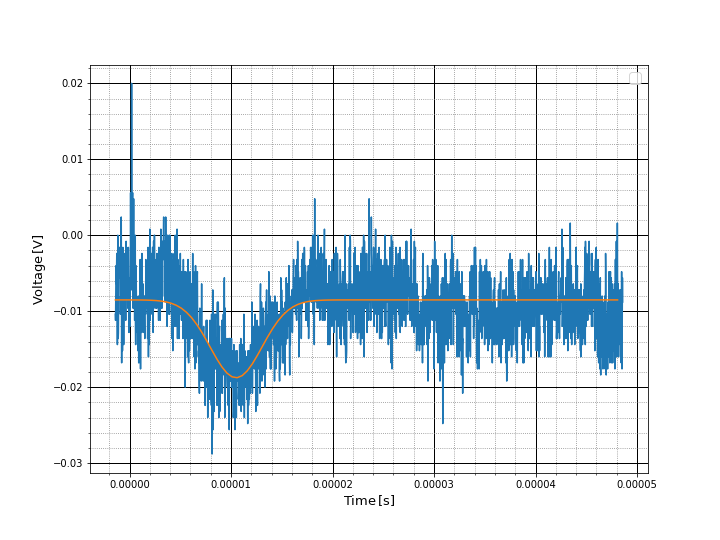
\includegraphics[scale=0.5]{Bild/A1}
	\centering
	\caption[Gaußfit an Messung bei Konst. Abstand]{Gaußfit an die Messungen der Elektronenwolken bei Konstantem Abstand von $3.6$\,mm und einer Spannung von $-15.2$\,V}
\end{figure}
\begin{figure}
	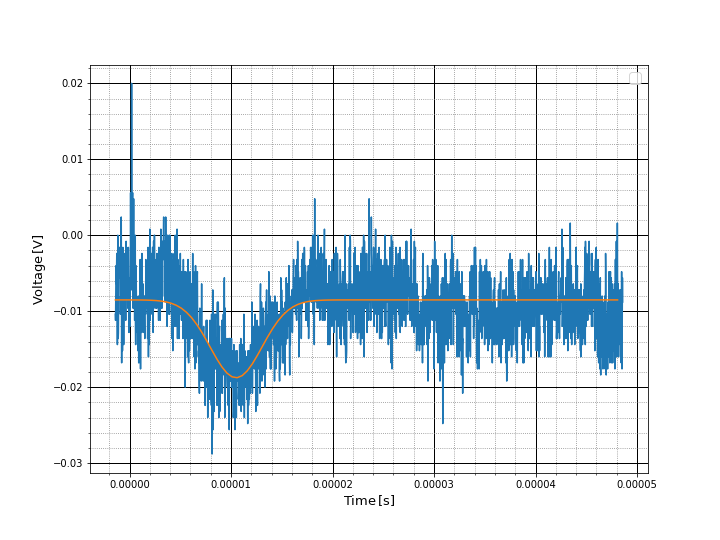
\includegraphics[scale=0.5]{Bild/A1}
	\centering
	\caption[Gaußfit an Messung bei Konst. Abstand]{Gaußfit an die Messungen der Elektronenwolken bei Konstantem Abstand von $3.6$\,mm und einer Spannung von $-18.4$\,V}
\end{figure}
\begin{figure}
	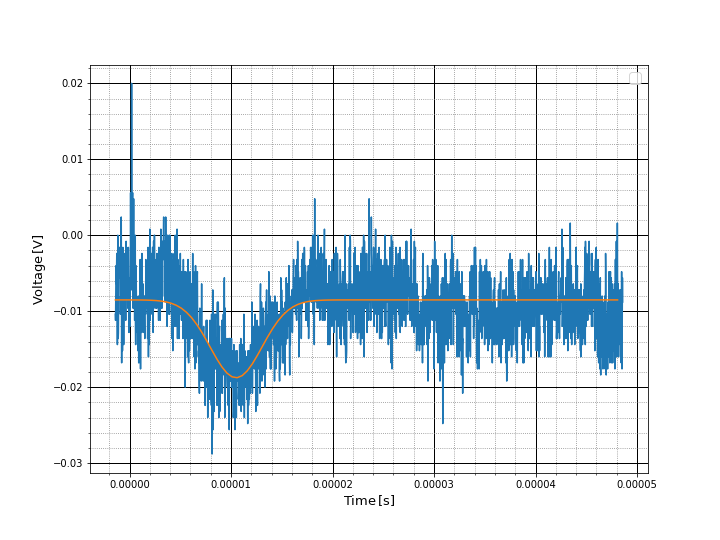
\includegraphics[scale=0.5]{Bild/A1}
	\centering
	\caption[Gaußfit an Messung bei Konst. Abstand]{Gaußfit an die Messungen der Elektronenwolken bei Konstantem Abstand von $3.6$\,mm und einer Spannung von $-20.4$\,V}
\end{figure}
\begin{figure}
	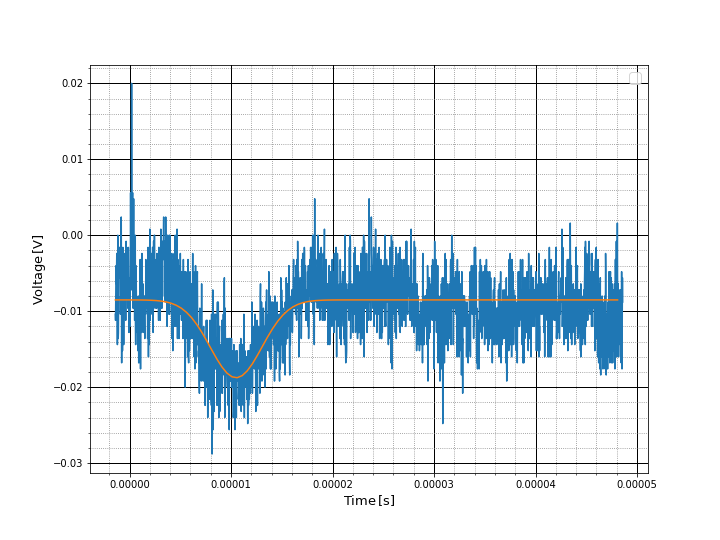
\includegraphics[scale=0.5]{Bild/A1}
	\centering
	\caption[Gaußfit an Messung bei Konst. Abstand]{Gaußfit an die Messungen der Elektronenwolken bei Konstantem Abstand von $3.6$\,mm und einer Spannung von $-22.4$\,V}
\end{figure}
\begin{figure}
	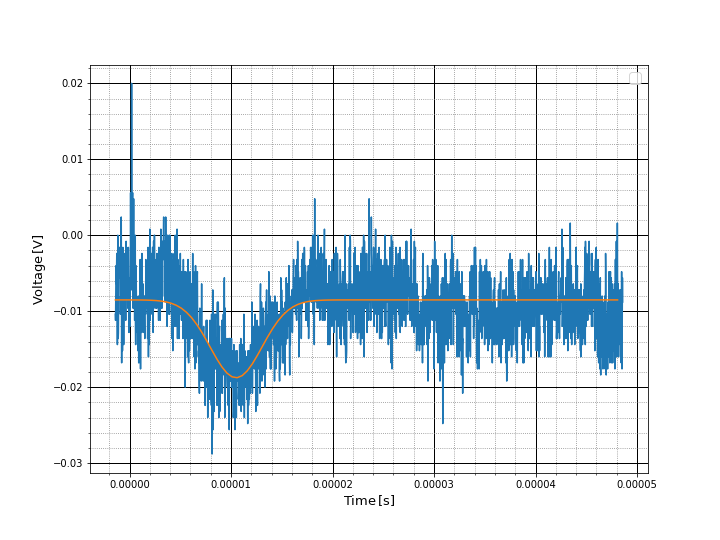
\includegraphics[scale=0.5]{Bild/A1}
	\centering
	\caption[Gaußfit an Messung bei Konst. Abstand]{Gaußfit an die Messungen der Elektronenwolken bei Konstantem Abstand von $3.6$\,mm und einer Spannung von $-24.4$\,V}
\end{figure}
\begin{figure}
	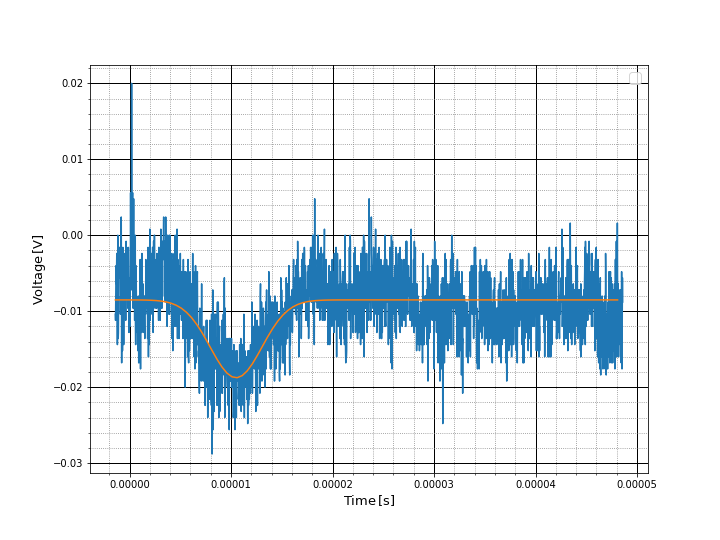
\includegraphics[scale=0.5]{Bild/A1}
	\centering
	\caption[Gaußfit an Messung bei Konst. Abstand]{Gaußfit an die Messungen der Elektronenwolken bei Konstantem Abstand von $3.6$\,mm und einer Spannung von $-28.0$\,V}
\end{figure}
\begin{figure}
	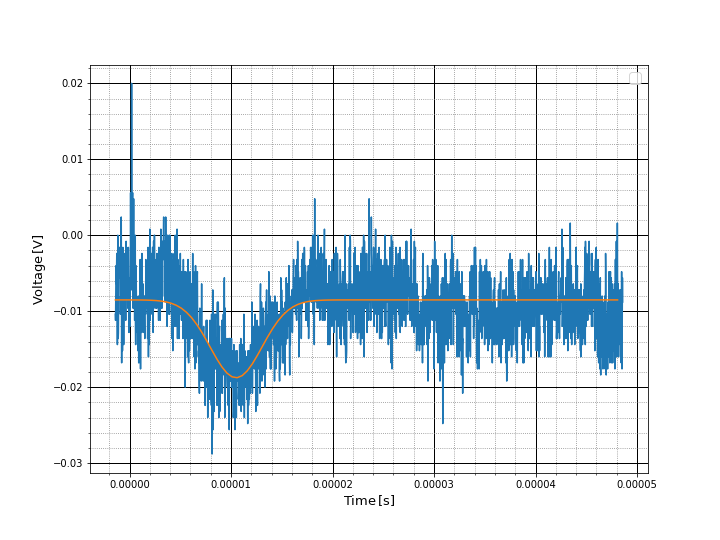
\includegraphics[scale=0.5]{Bild/A1}
	\centering
	\caption[Gaußfit an Messung bei Konst. Abstand]{Gaußfit an die Messungen der Elektronenwolken bei Konstantem Abstand von $3.6$\,mm und einer Spannung von $-32.0$\,V}
\end{figure}
\begin{figure}
	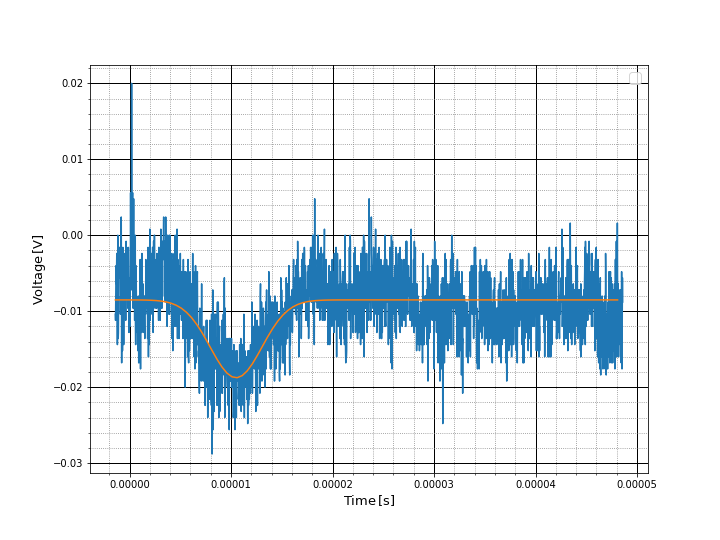
\includegraphics[scale=0.5]{Bild/A1}
	\centering
	\caption[Gaußfit an Messung bei Konst. Abstand]{Gaußfit an die Messungen der Elektronenwolken bei Konstantem Abstand von $3.6$\,mm und einer Spannung von $-36.0$\,V}
\end{figure}
\begin{figure}
	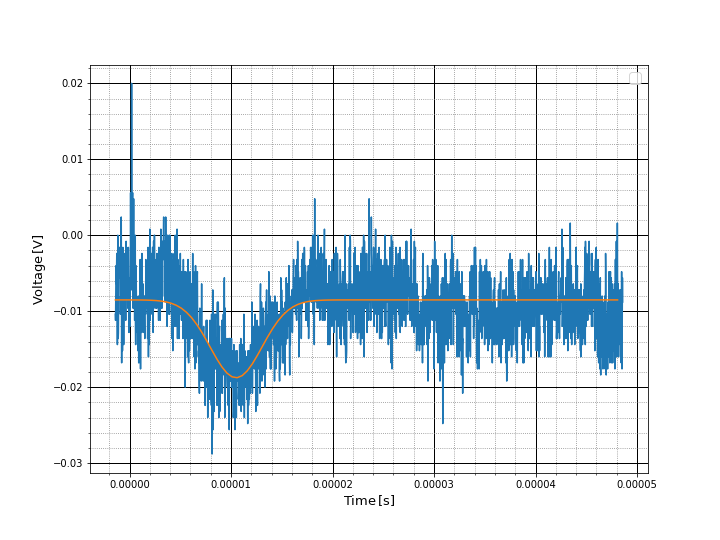
\includegraphics[scale=0.5]{Bild/A1}
	\centering
	\caption[Gaußfit an Messung bei Konst. Abstand]{Gaußfit an die Messungen der Elektronenwolken bei Konstantem Abstand von $3.6$\,mm und einer Spannung von $-40.0$\,V}
\end{figure}
\begin{figure}
	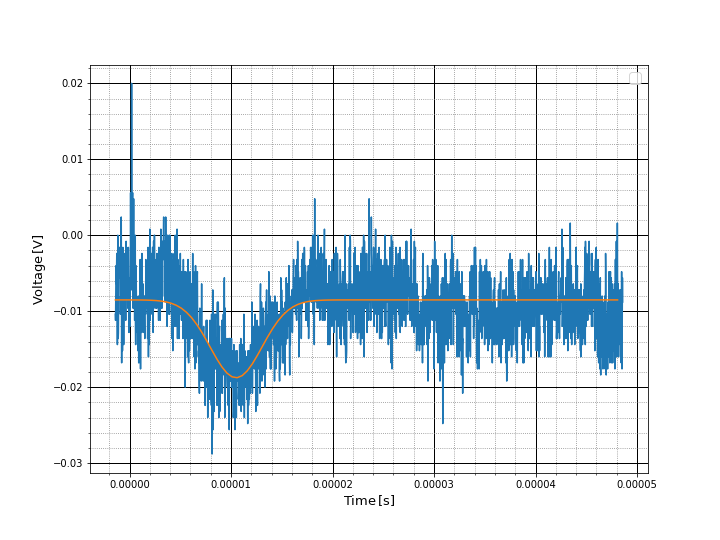
\includegraphics[scale=0.5]{Bild/A1}
	\centering
	\caption[Gaußfit an Messung bei Konst. Abstand]{Gaußfit an die Messungen der Elektronenwolken bei Konstantem Abstand von $3.6$\,mm und einer Spannung von $-44.0$\,V}
\end{figure}
\begin{figure}
	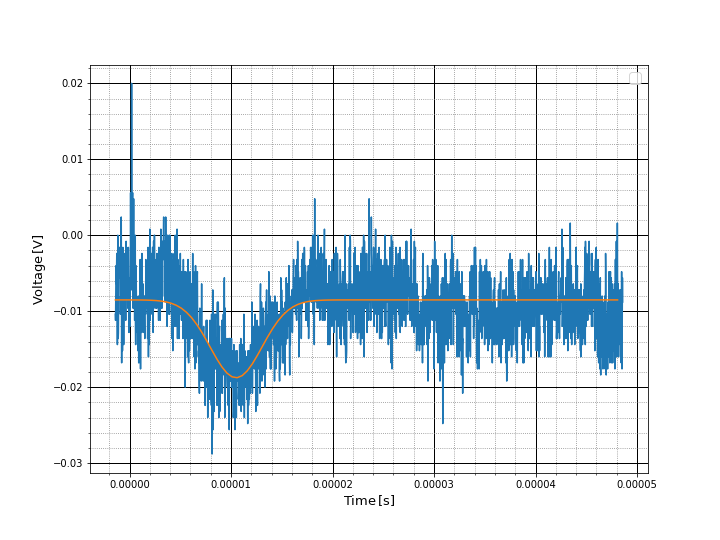
\includegraphics[scale=0.5]{Bild/A1}
	\centering
	\caption[Gaußfit an Messung bei Konst. Abstand]{Gaußfit an die Messungen der Elektronenwolken bei Konstantem Abstand von $3.6$\,mm und einer Spannung von $-46.0$\,V}
\end{figure}
\begin{figure}
	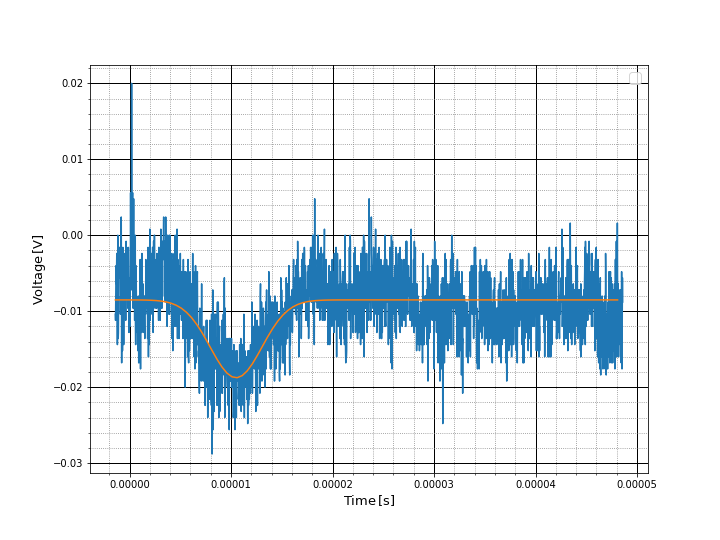
\includegraphics[scale=0.5]{Bild/A1}
	\centering
	\caption[Gaußfit an Messung bei Konst. Abstand]{Gaußfit an die Messungen der Elektronenwolken bei Konstantem Abstand von $3.6$\,mm und einer Spannung von $-48.0$\,V}
\end{figure}

%Lange Messungen

\begin{figure}[ht]
	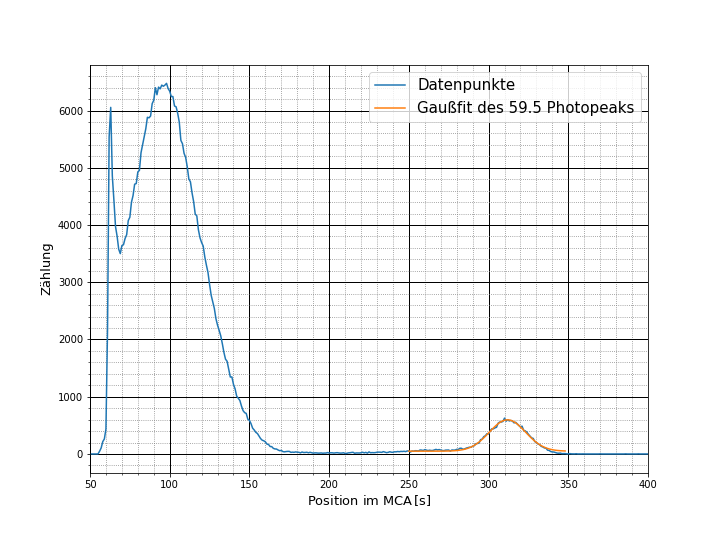
\includegraphics[scale=0.5]{Bild/ASg}
	\centering
	\caption{Gesamtes Spektrum von Americium mit Silizium aufgenommen.}
\end{figure}
\begin{figure}[ht]
	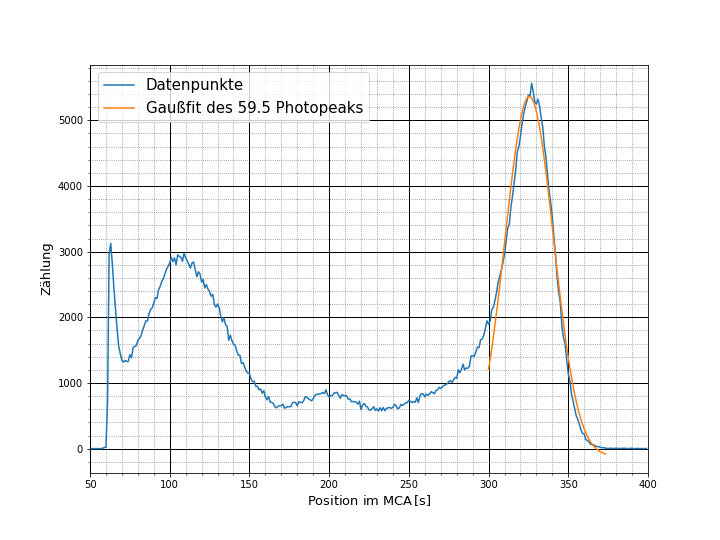
\includegraphics[scale=0.5]{Bild/ACg}
	\centering
	\caption{Gesamtes Spektrum von Americium mit CdTe aufgenommen.}
\end{figure}
\begin{figure}[ht]
	\includegraphics[scale=0.5]{Bild/CSg}
	\centering
	\caption{Gesamtes Spektrum von Cobalt mit Silizium aufgenommen.}
\end{figure}
\begin{figure}[ht]
	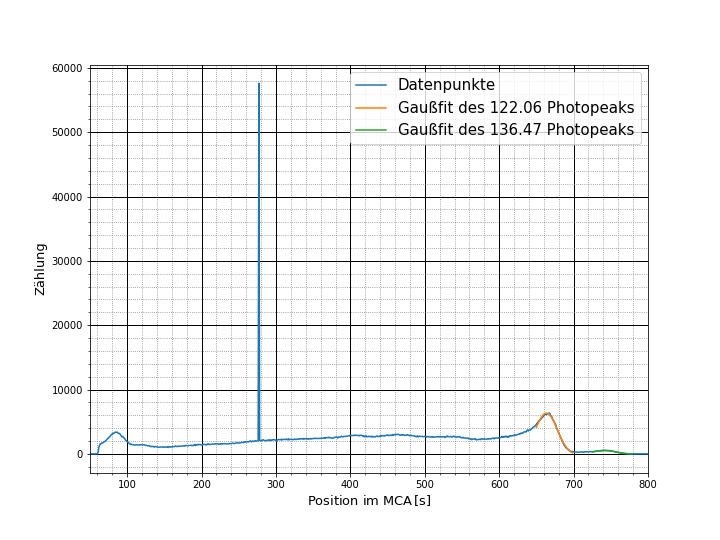
\includegraphics[scale=0.5]{Bild/CCg}
	\centering
	\caption{Gesamtes Spektrum von Cobalt mit CdTe aufgenommen.}
\end{figure}
\subsection{Laborbuch}
%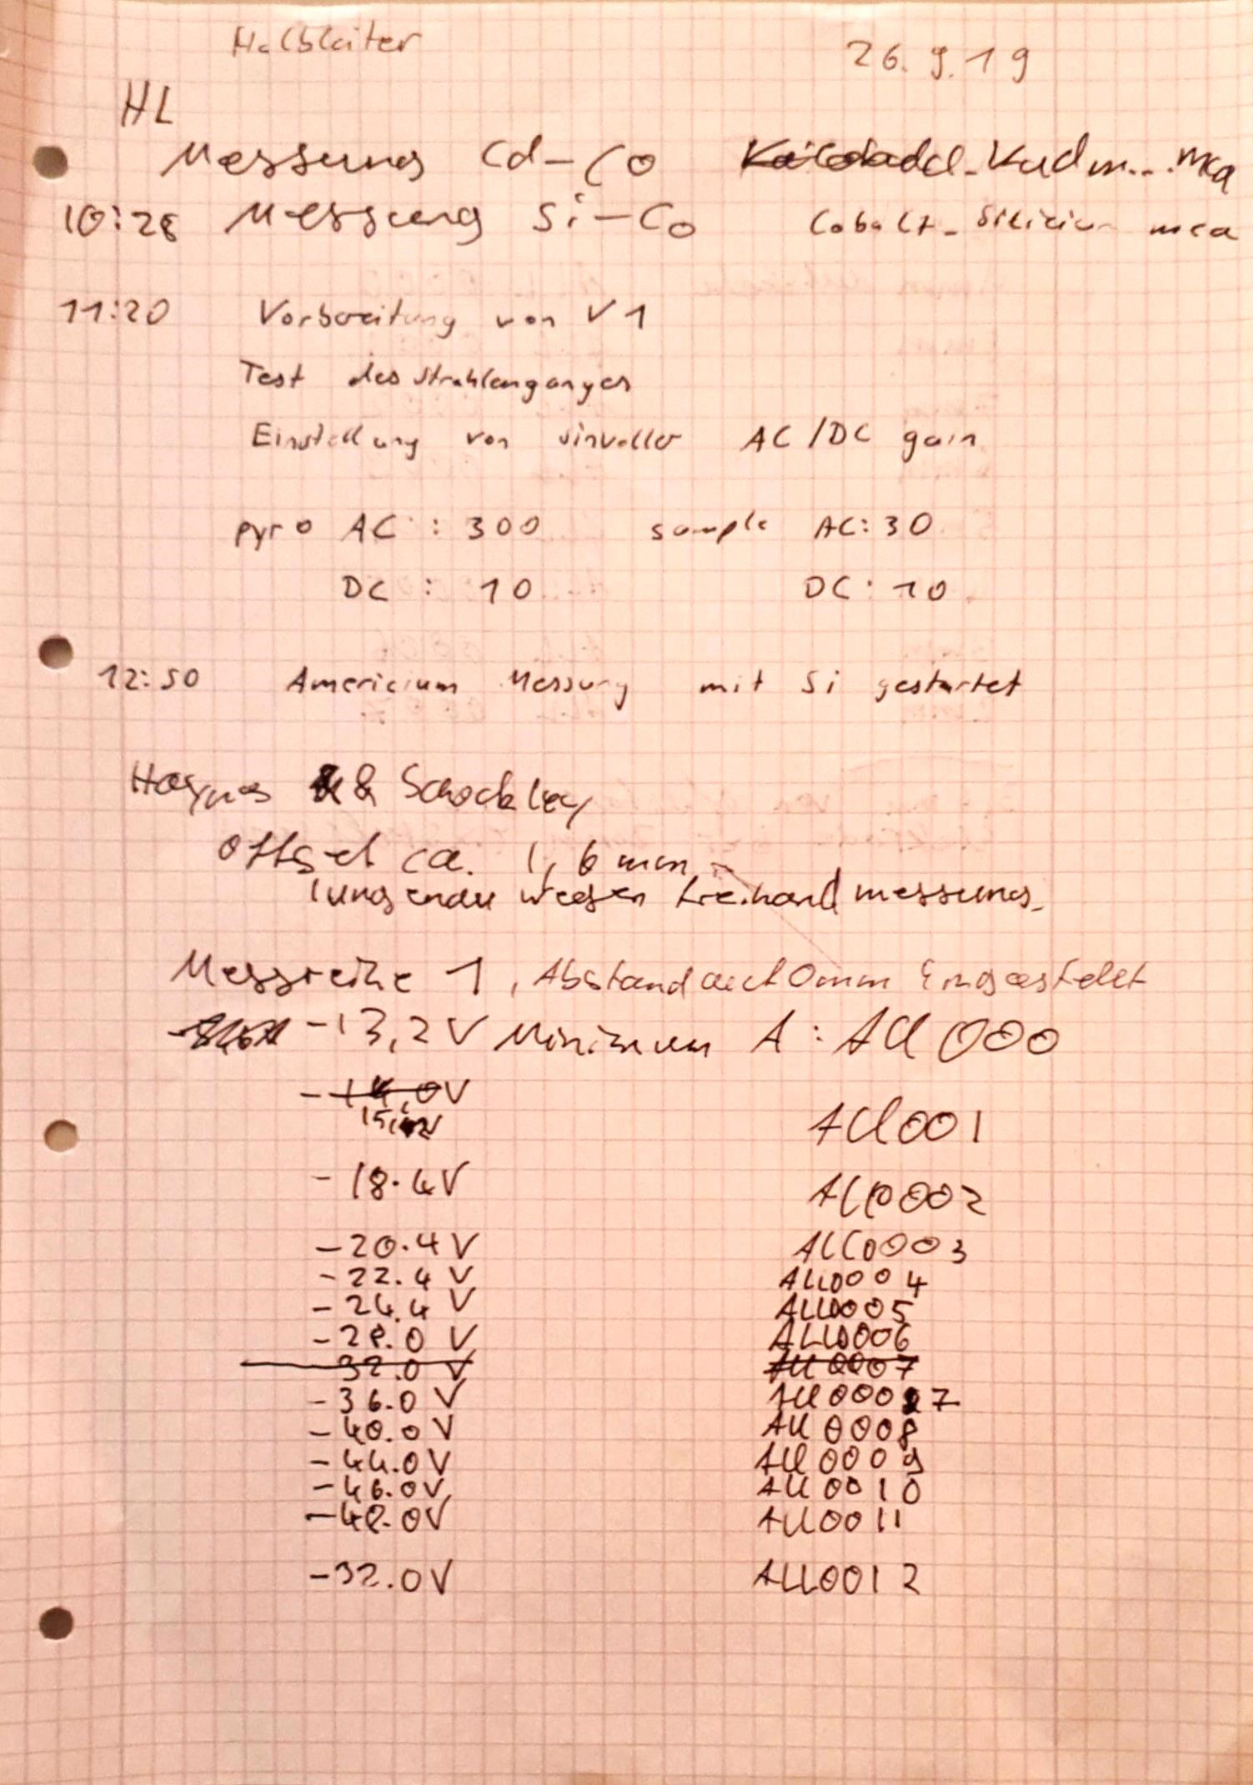
\includepdf[pages=-,scale=0.8]{Bilder/anhang/Halbleiter.pdf}
\end{document}